\label{sec:fake_photons_background}
The background from fake photons, either misidentified or \nonprompt, can be estimated using a similar data-driven approach.
It is necessary to define two working points, one being the loose selection and the other the tight analysis selection.
For this analysis, the Loose working point of the cut-based ID is the tight analysis selection,
while the \textit{very loose} selection (see Section \ref{sec:photon_selection}) is used as the loose criterion.
The differences between the two selections are the two cuts on \sieie and H/E, which have a good discriminating power against \nonprompt photons and misidentified jets.

\subsubsection{Photon fake rate measurement}
The photon fake rate measurement, which is the probability for a fake photon that passes the loose selection to also pass the tight one,
is done on a subset of the same $\PZ+L$ region that is used for the lepton fake rate.
In addition to the requirements for that region, events must also have a photon with $\pt > 20 \GeV$ and $|\eta| < 1.4442$ or $1.556 < |\eta| < 2.4$
which passes the loose selection.
The photon must have a distance from any of the three leptons of $\DR(\PGg, \Pl) > 0.5$.
In case there is more than one photon passing the requirements, the one with the highest \pt is selected.

The main processes in the fake rate measurement region are Drell-Yan and $\PZ\PGg$, as can be seen in Figure \ref{fig:CRLFR_inclusive}.
The latter contains prompt photons, which would bias the result of the measurement, and thus must be removed.
Events in the $\PZ\PGg$ sample which have a generator level prompt photon that is matched within $\DR(\PGg^{GEN}, \PGg^{REC}) < 0.2$ are considered prompt.
Prompt events are subtracted from the data, in the appropriate bins of \pt and pseudorapidity of the photon,
both from the numerator (photons that pass the selection, Figure~\ref{fig:CRLFR_lead_pass})
and from the denominator, which is the sum of the passing and the failing (Figure~\ref{fig:CRLFR_lead_fail}) photons.

\begin{figure}
  \centering
  \subfigure [$m_{\PZ\Pl}$] {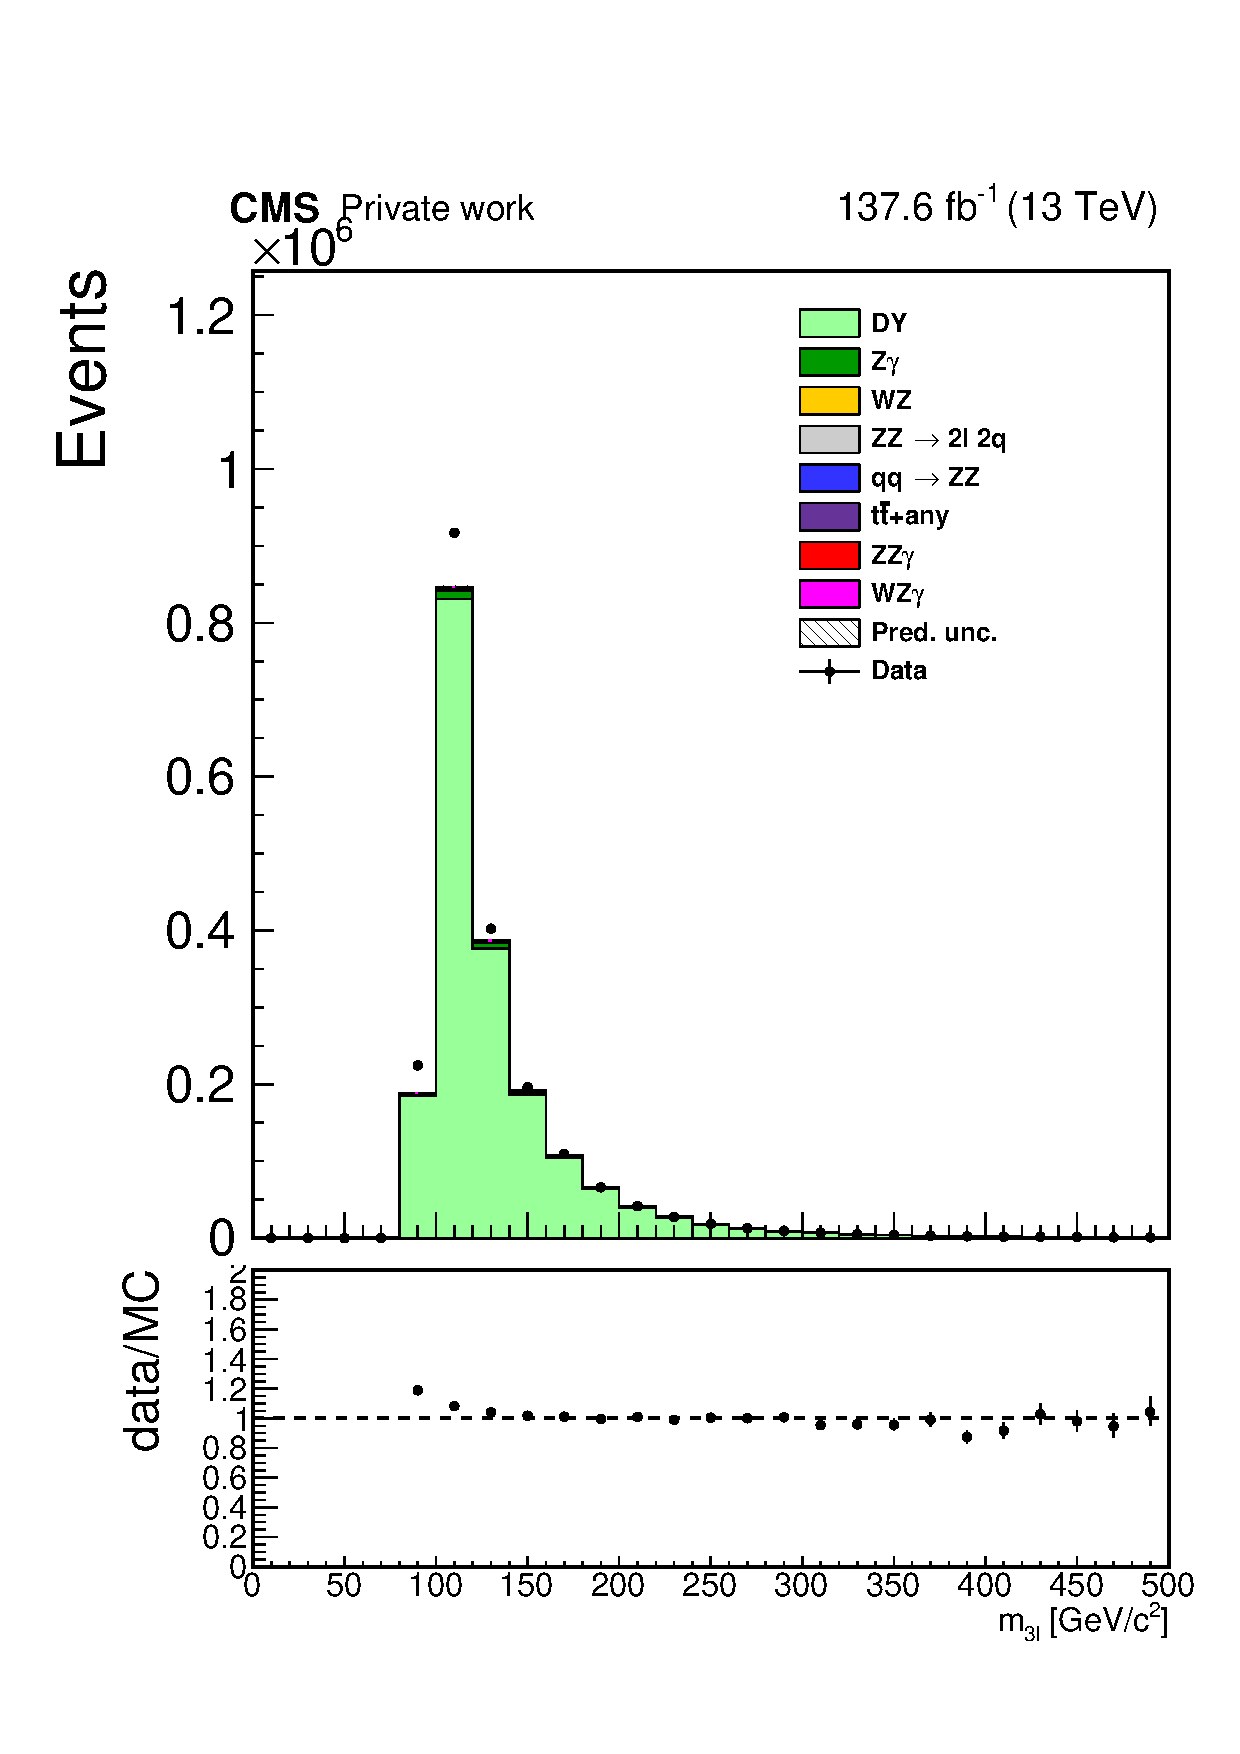
\includegraphics[width=.333333333\textwidth]{dataMC/Run2/fullMC/CRLFR/ZL_mass_pow.pdf}}%
  \subfigure [$\pt$ of $\Pl^0$] {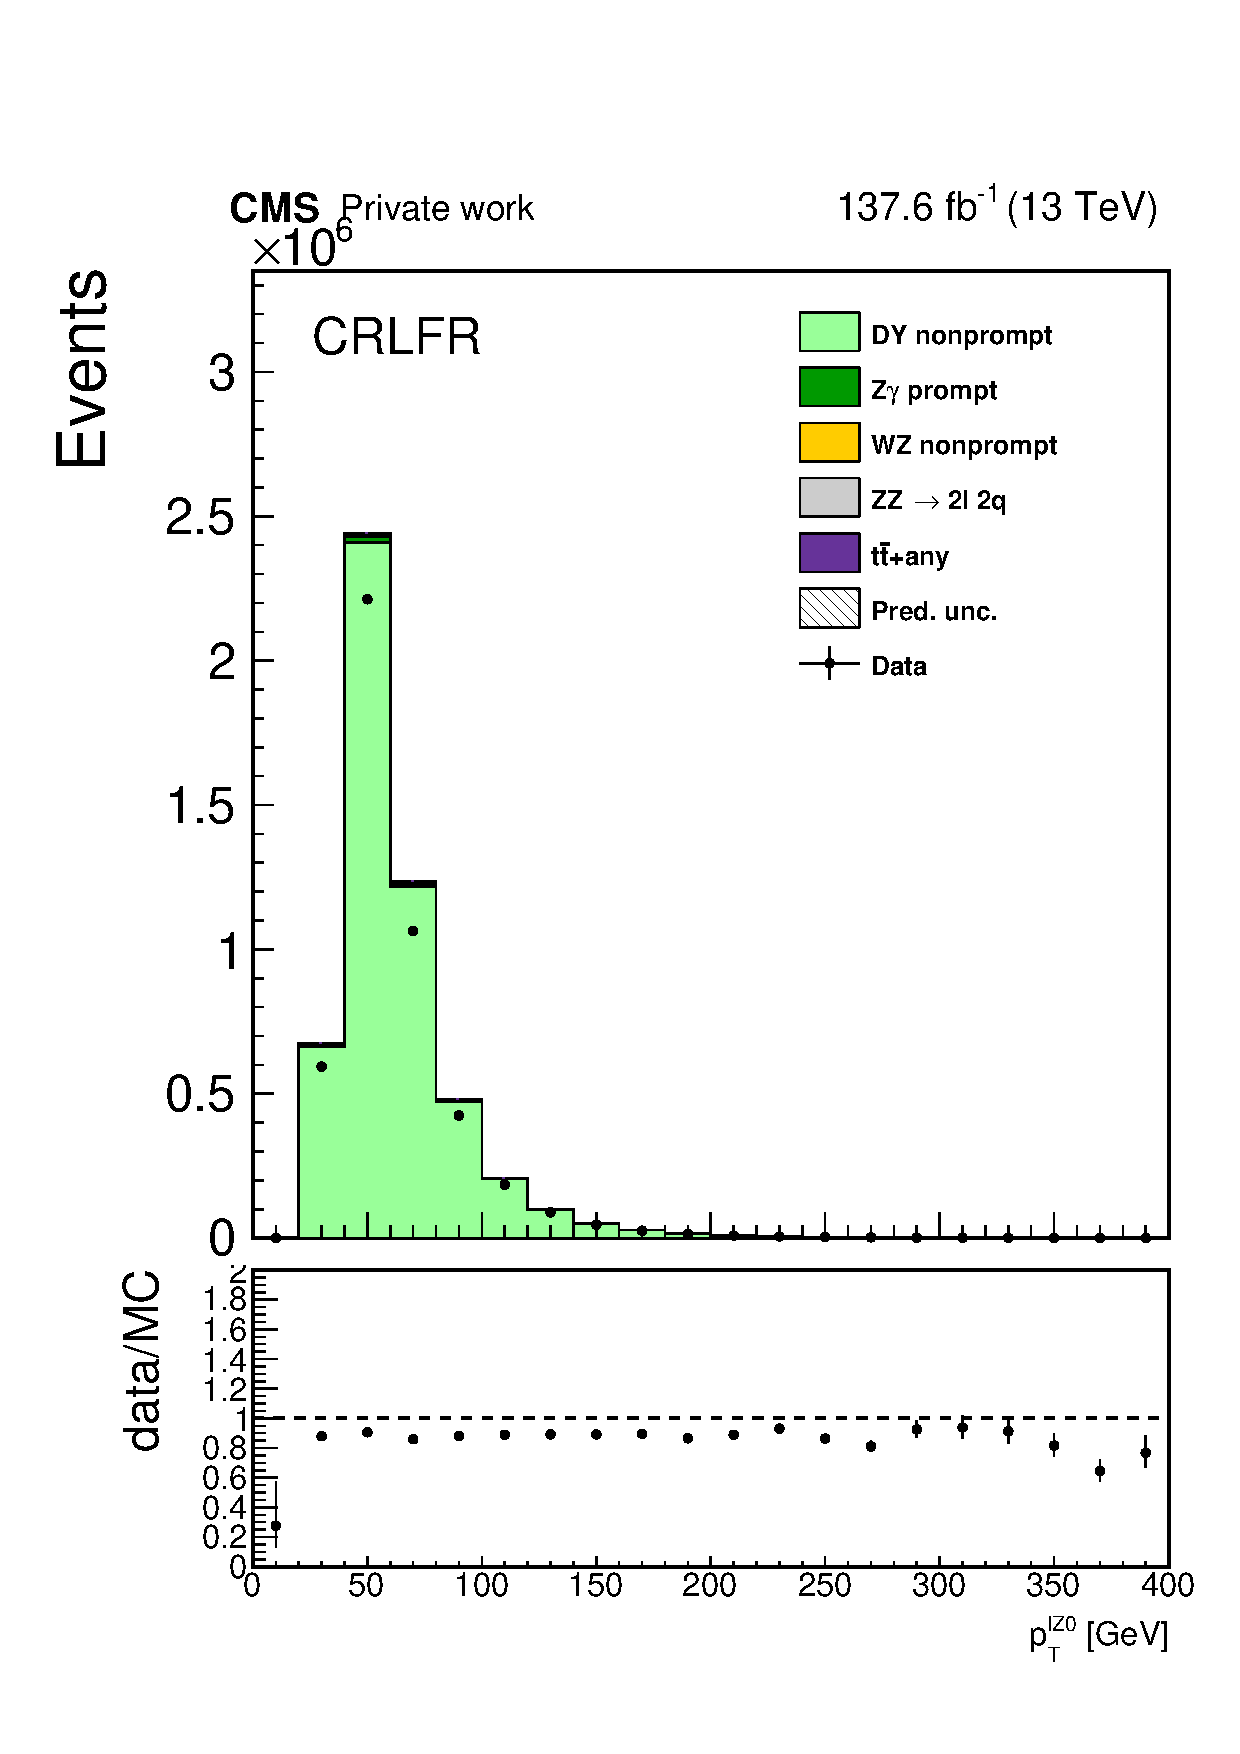
\includegraphics[width=.333333333\textwidth]{dataMC/Run2/fullMC/CRLFR/Z_l0_pt_pow.pdf}}%
  \subfigure [Number of $\PGg^{\rm kinematic}$] {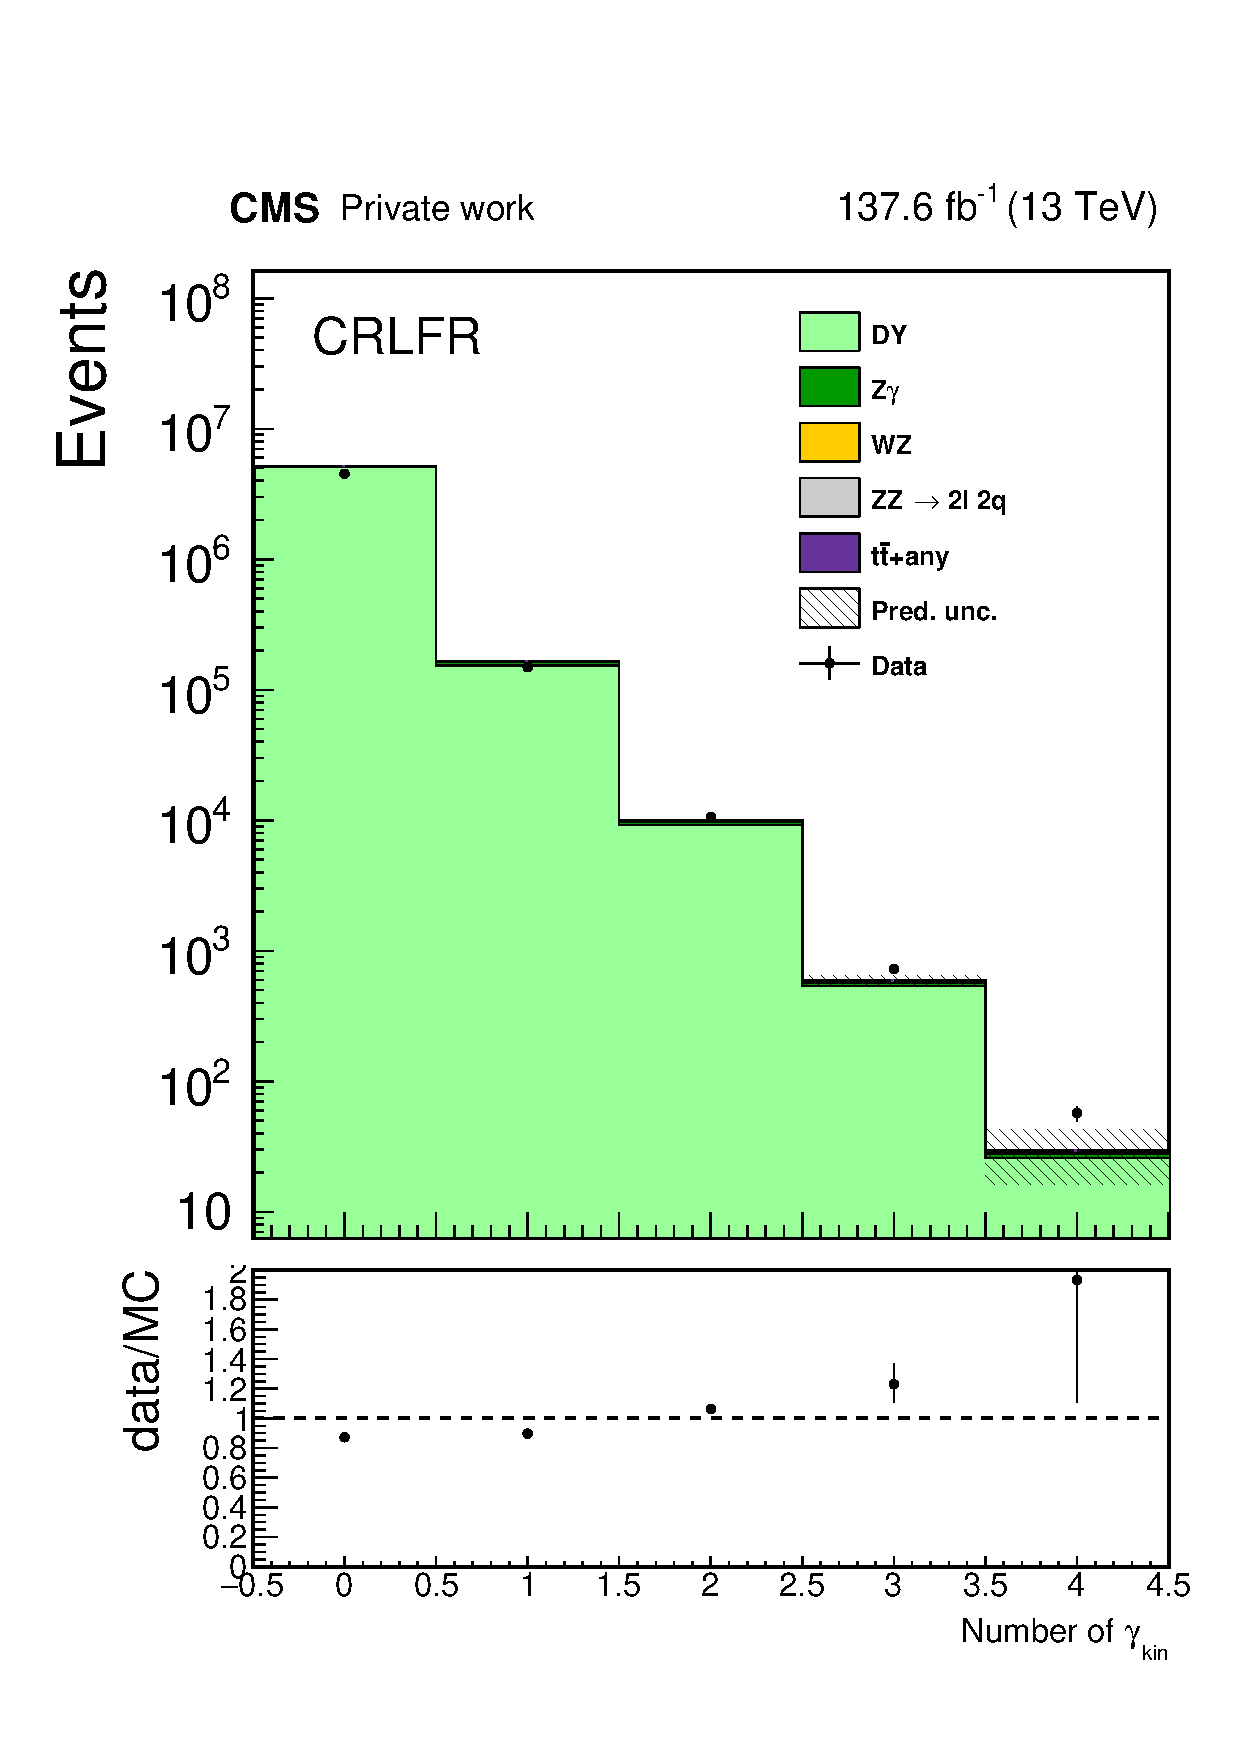
\includegraphics[width=.333333333\textwidth]{dataMC/Run2/fullMC/CRLFR/kinPh_central_N_pow.pdf}}
  \caption{Invariant mass of the three lepton system (left),
    transverse momentum of the leading lepton from the Z candidate (centre)
    and number of photon passing the kinematic selection (right)
    in the fake rate measurement region, integrated on the whole \Run2 period.}
  \label{fig:CRLFR_inclusive}
\end{figure}

\begin{figure}
  \centering
  \subfigure [$\pt   $ of $\PGg^{\rm fail}$] {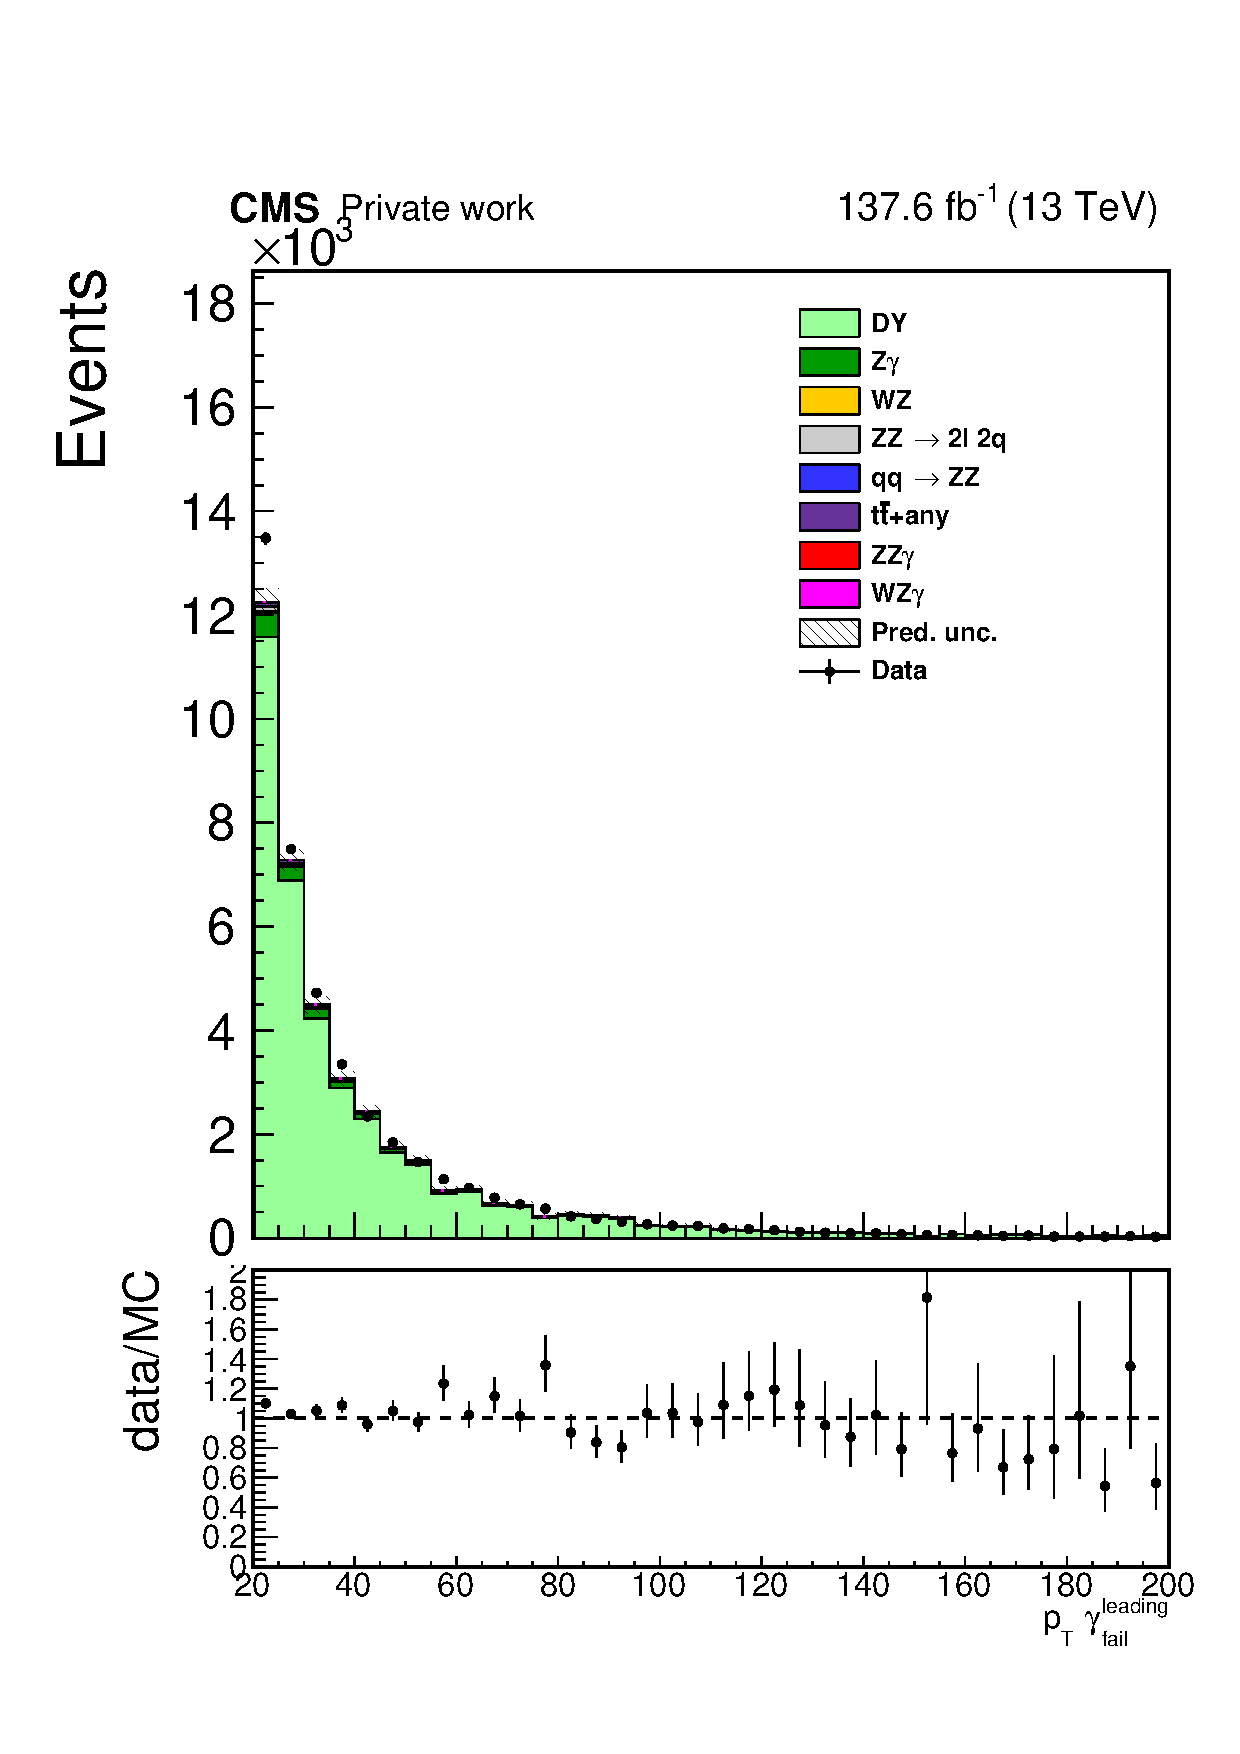
\includegraphics[width=.333333333\textwidth]{dataMC/Run2/fullMC/CRLFR/lead_fail_pt_fine_pow.pdf}}%
  \subfigure [$|\eta|$ of $\PGg^{\rm fail}$] {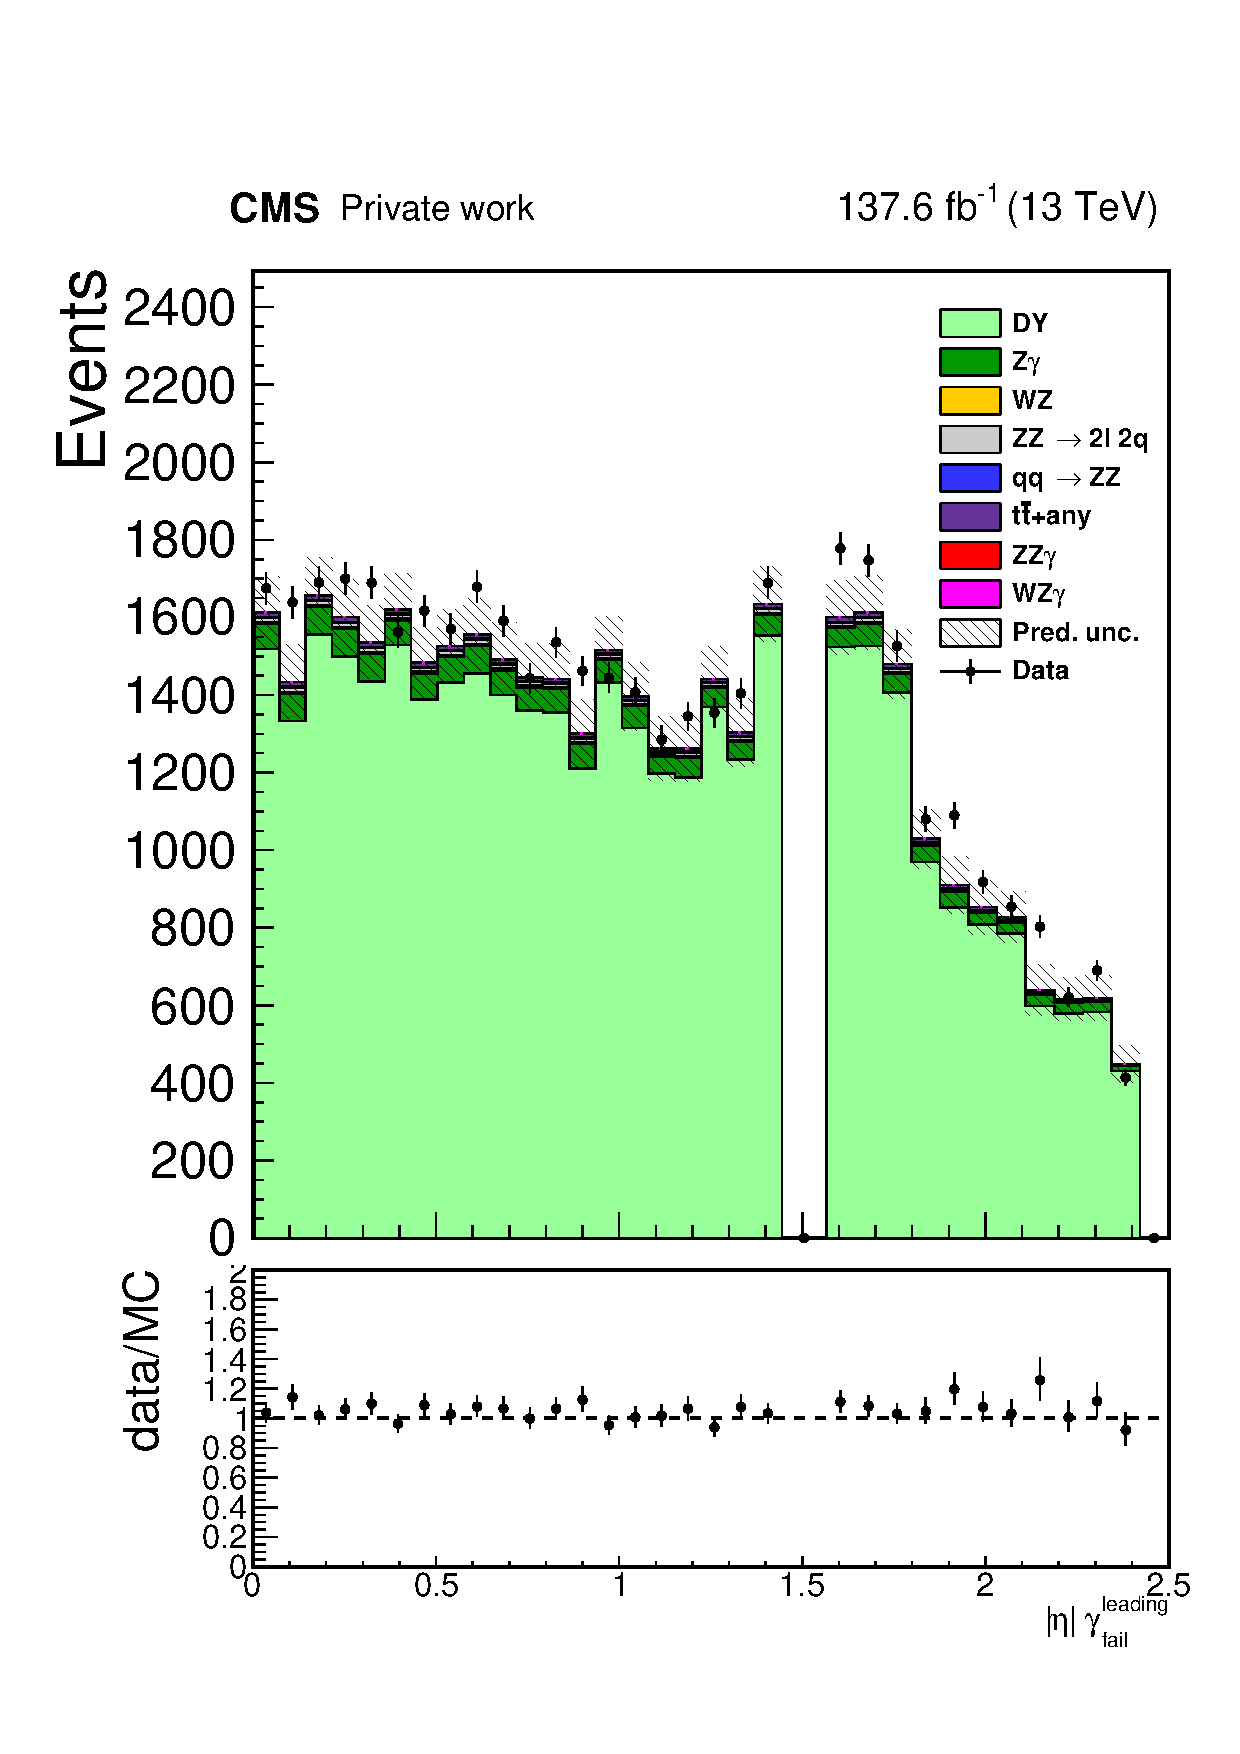
\includegraphics[width=.333333333\textwidth]{dataMC/Run2/fullMC/CRLFR/lead_fail_aeta_fine_pow.pdf}}%
  \subfigure [$\sieie$ of $\PGg^{\rm fail}$] {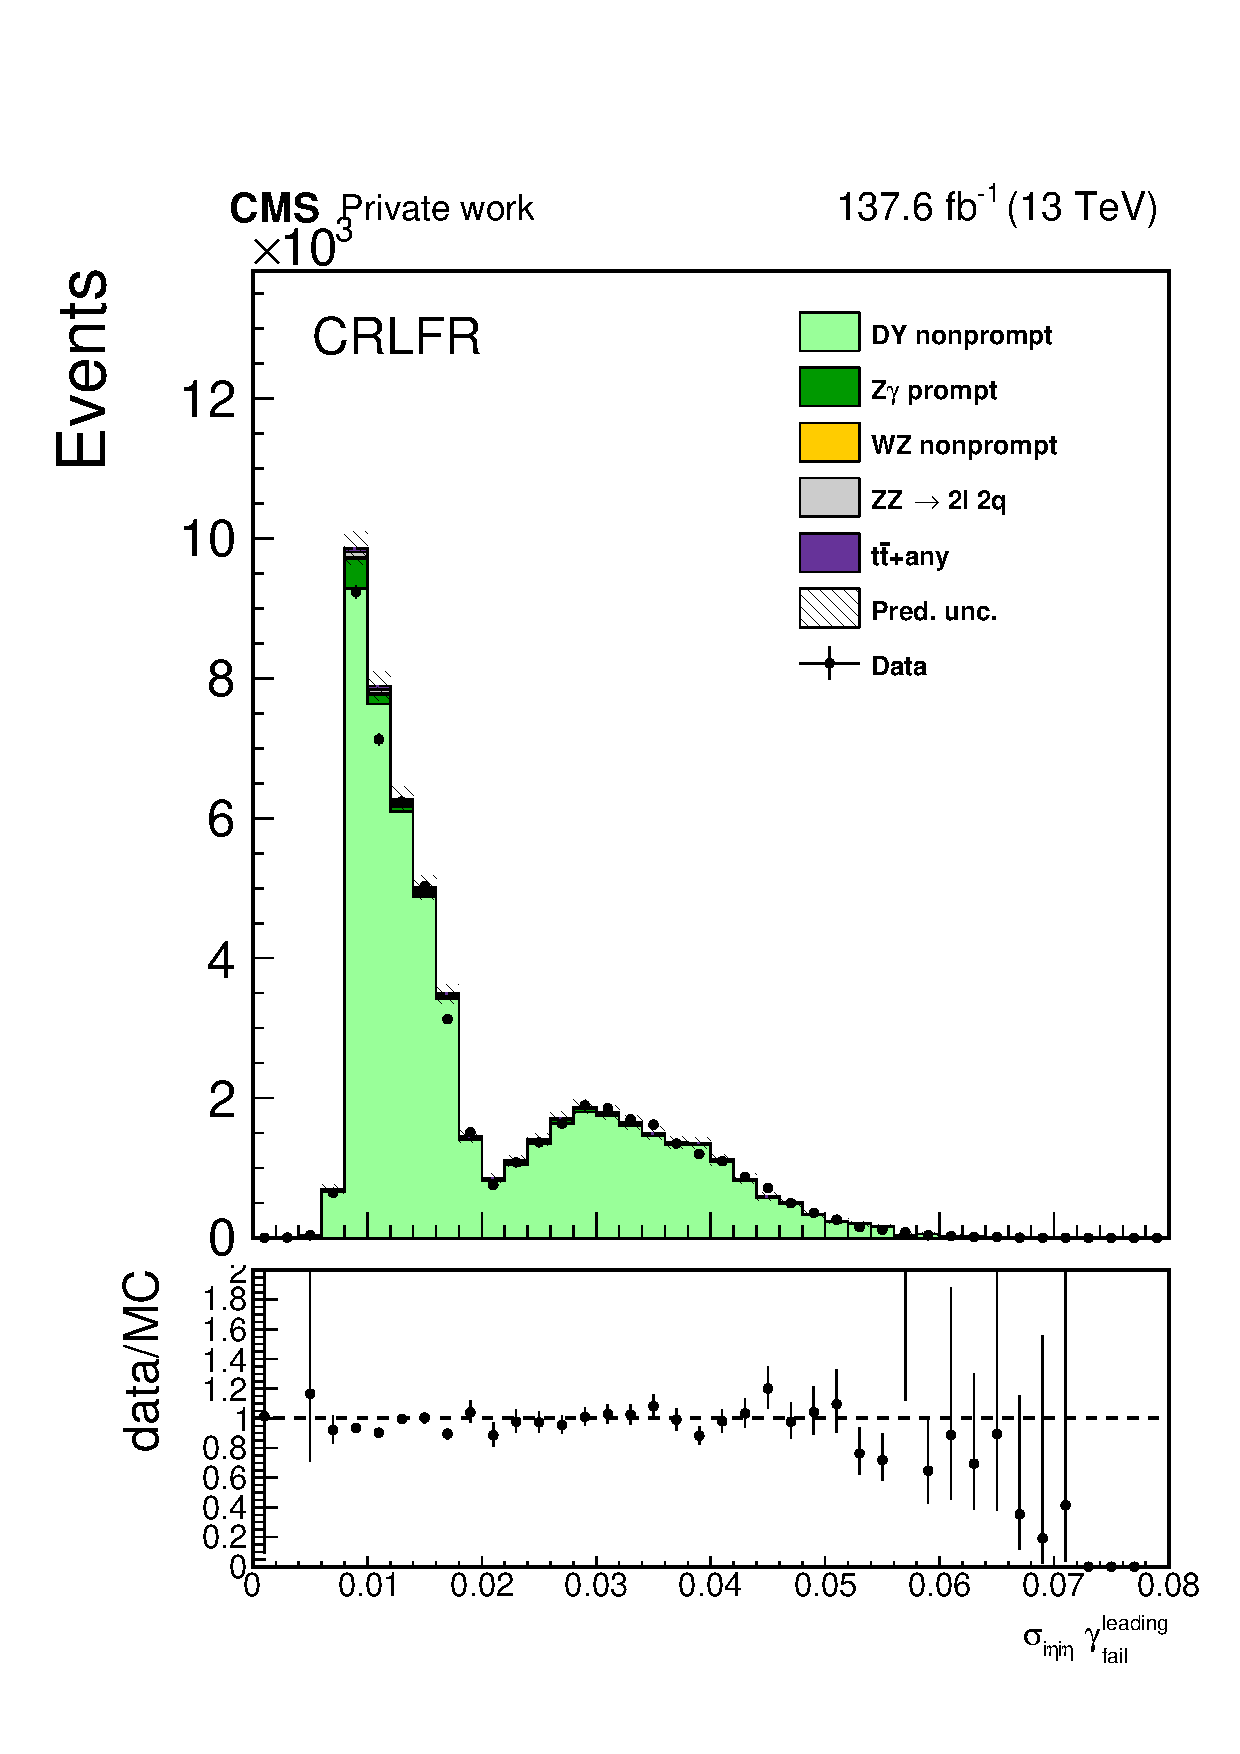
\includegraphics[width=.333333333\textwidth]{dataMC/Run2/fullMC/CRLFR/lead_fail_sieie_pow.pdf}}
  \caption{Transverse momentum, pseudorapidity and \sieie of photons
    passing the loose criterion (VeryLoose ID) but failing the tight selection (Loose working point of the cut-based ID)
    in the fake rate measurement region, integrated on the whole \Run2 period.}
  \label{fig:CRLFR_lead_fail}
\end{figure}

\begin{figure}
  \centering
  \subfigure [$\pt   $ of $\PGg^{\rm pass}$] {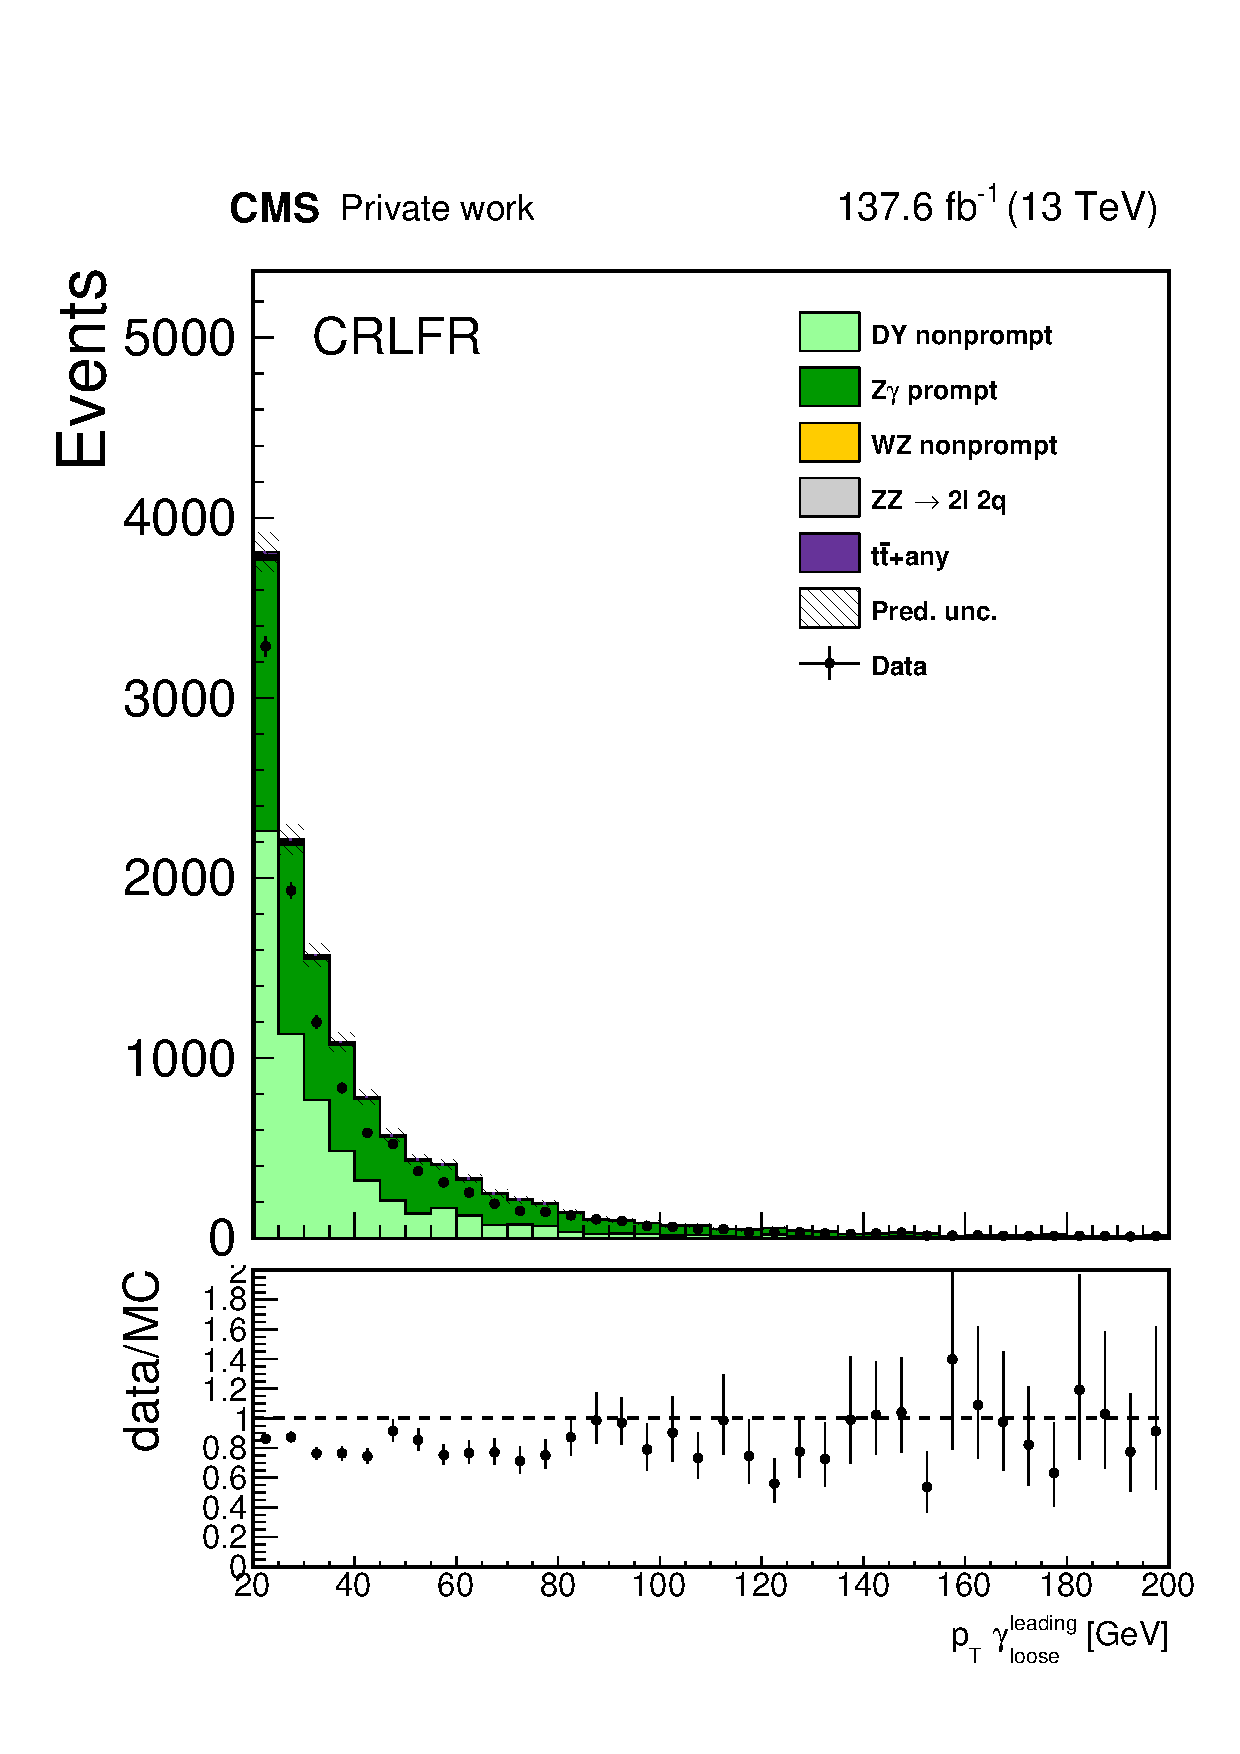
\includegraphics[width=.333333333\textwidth]{VVGammaAnalyzer/Run2/fullMC/CRLFR/lead_loose_pt_fine_pow.pdf}}%
  \subfigure [$|\eta|$ of $\PGg^{\rm pass}$] {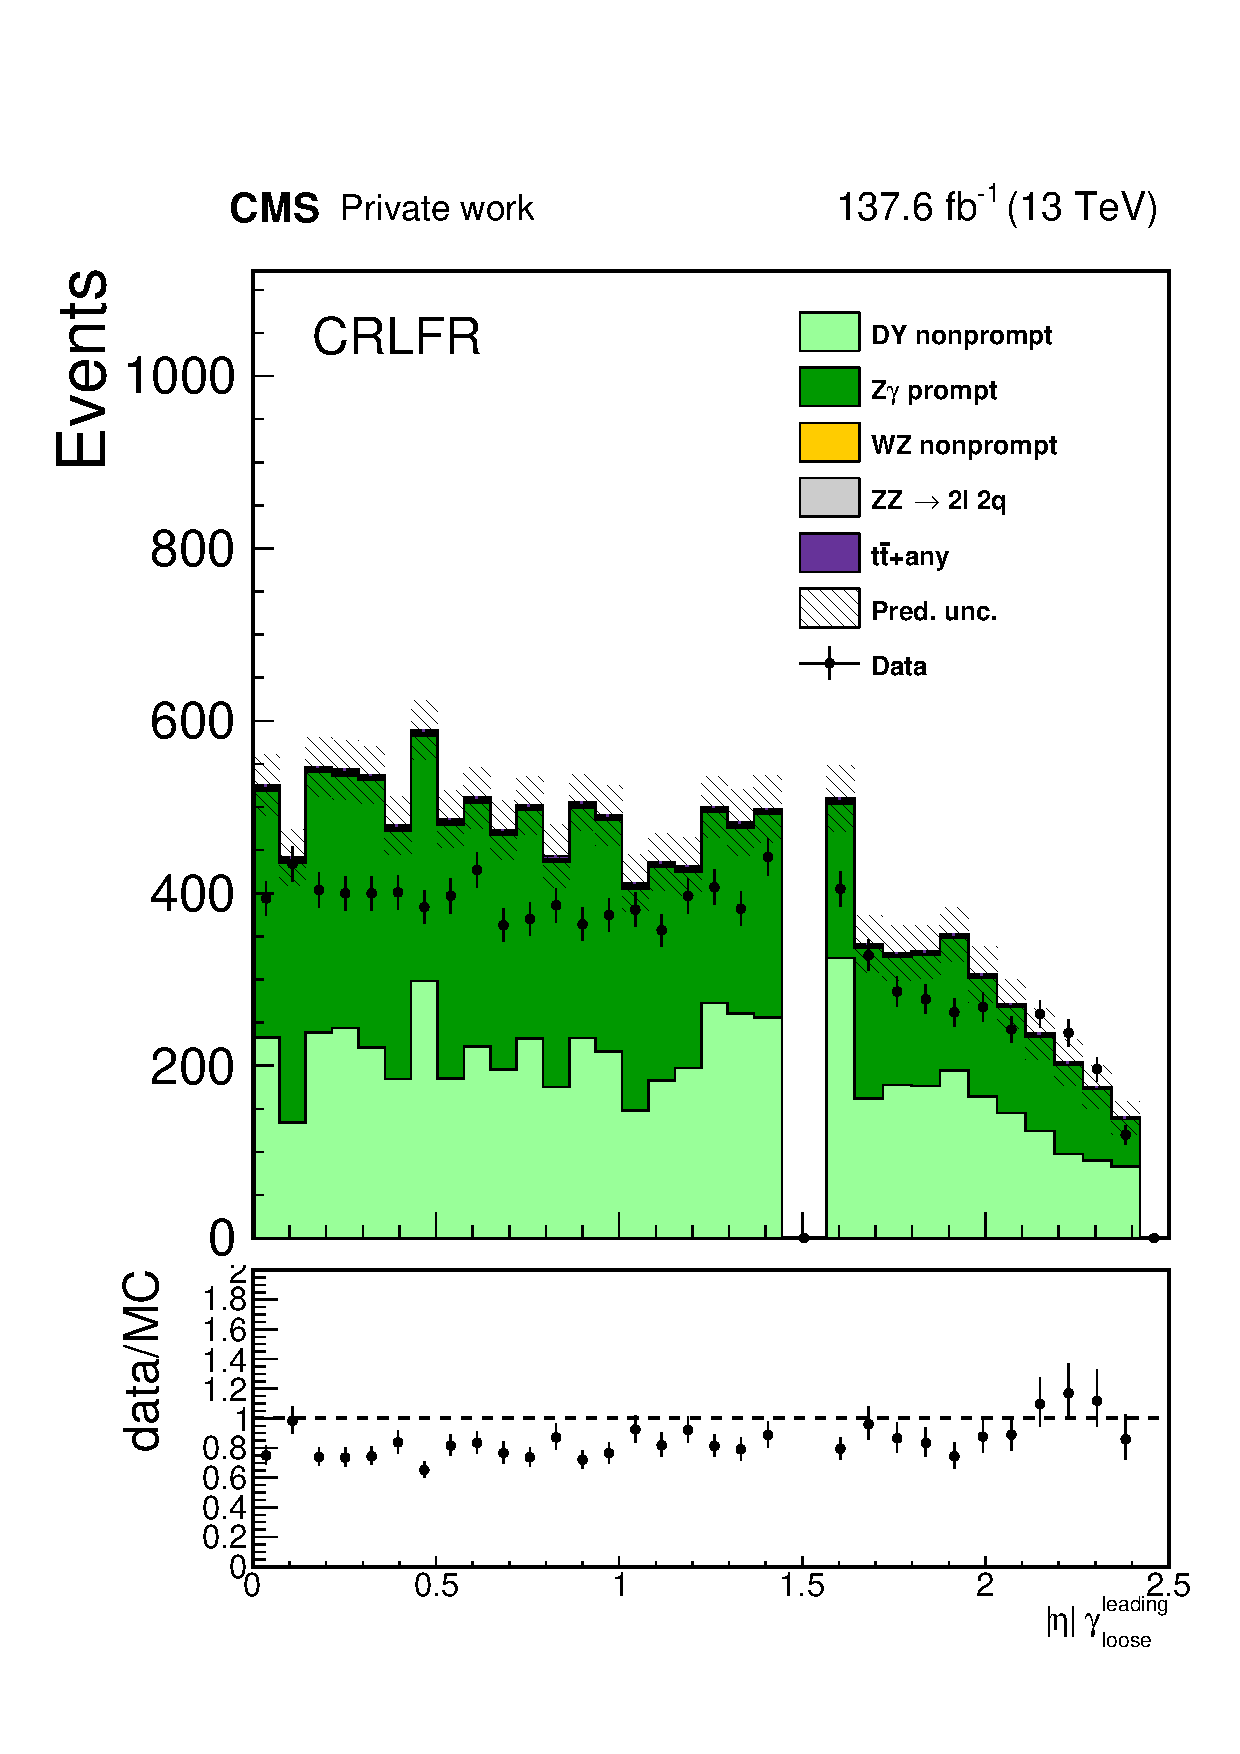
\includegraphics[width=.333333333\textwidth]{VVGammaAnalyzer/Run2/fullMC/CRLFR/lead_loose_aeta_fine_pow.pdf}}%
  \subfigure [$\sieie$ of $\PGg^{\rm pass}$] {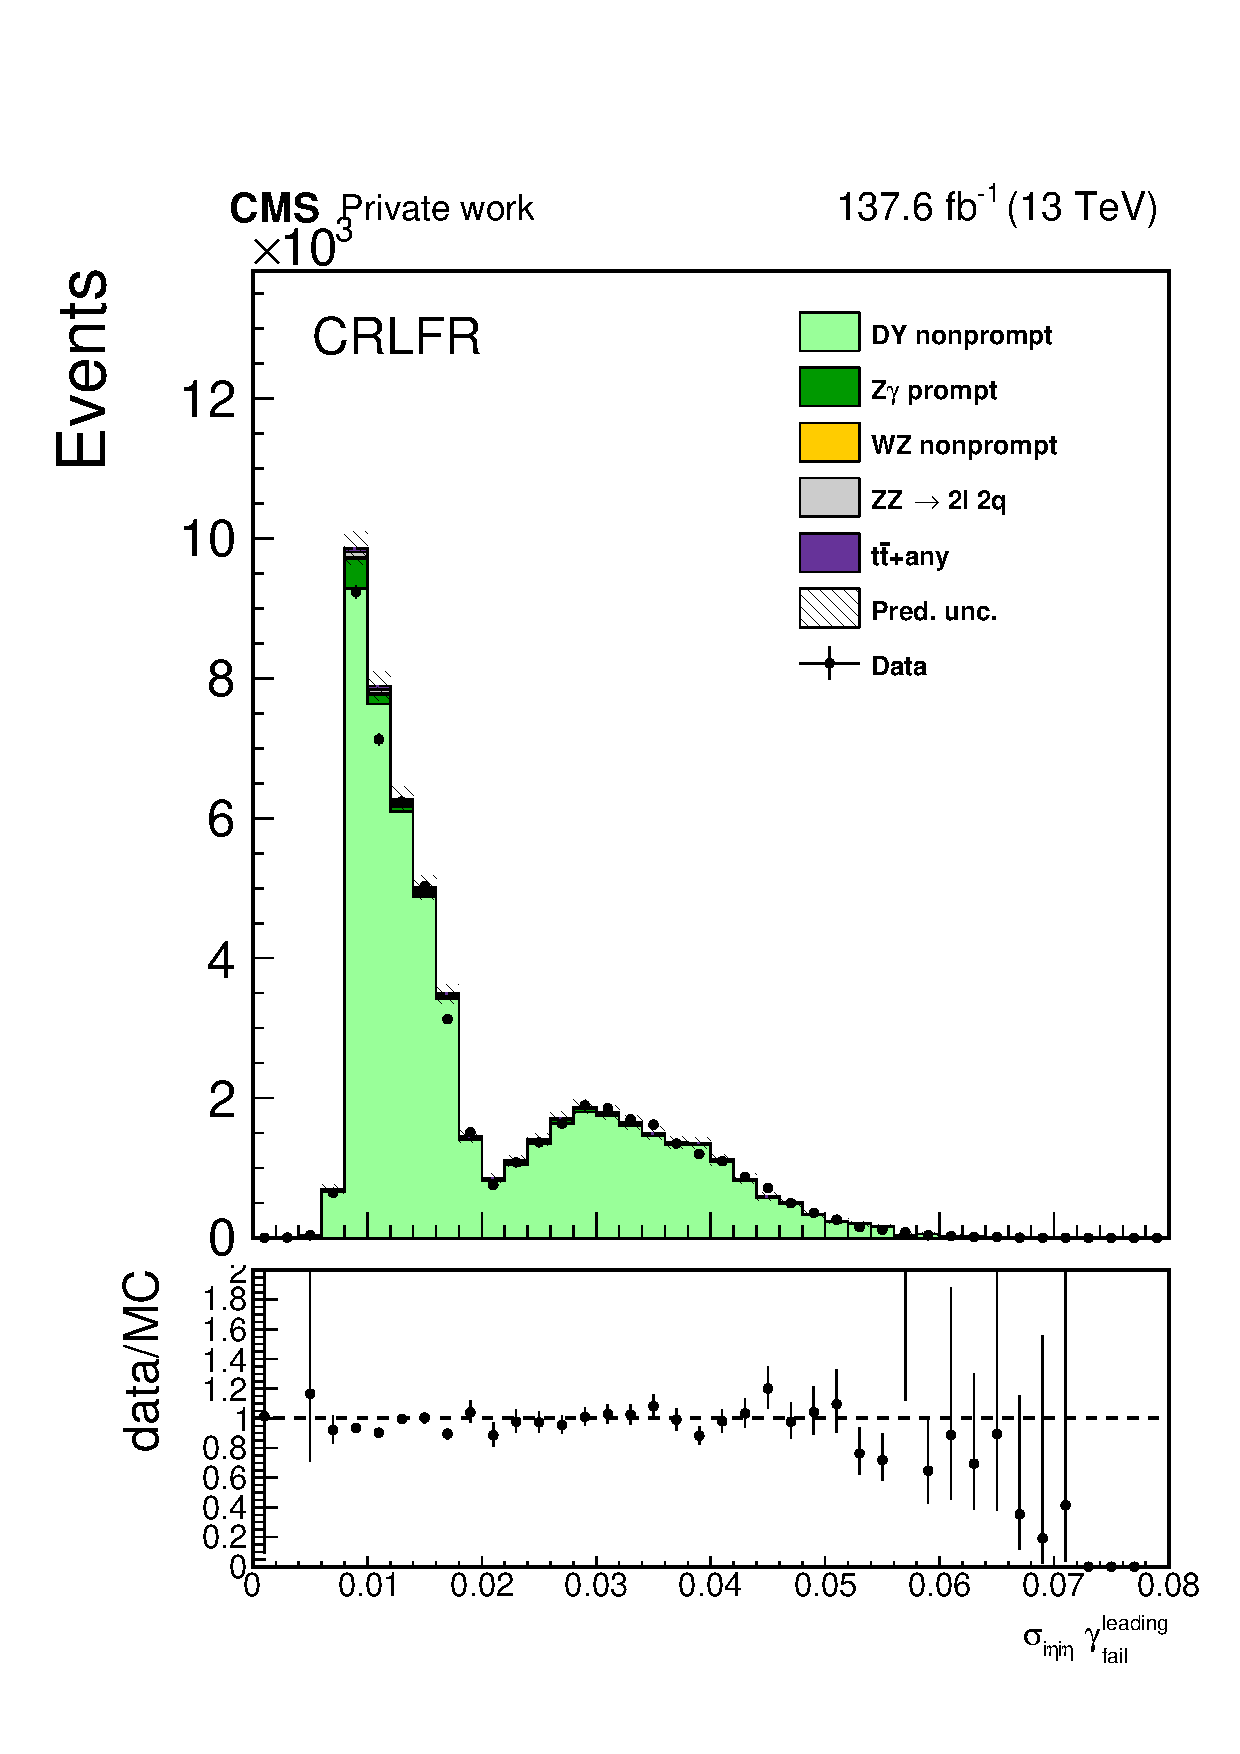
\includegraphics[width=.333333333\textwidth]{dataMC/Run2/fullMC/CRLFR/lead_fail_sieie_pow.pdf}}
  \caption{Transverse momentum, pseudorapidity and \sieie of photons
    passing the tight selection (Loose working point of the cut-based ID)
    in the fake rate measurement region, integrated on the whole \Run2 period.}
  \label{fig:CRLFR_lead_pass}
\end{figure}

The fake rate is then measured as the ratio of events in which the photon passes also the tight selection (the Loose working point of the cut-based ID)
to the total.
This measurement is done separately for endcap and barrel, for several bins of \pt (Figure \ref{fig:phFR_VLtoL}).

\begin{figure}
\subfigure [2016preVFP ] {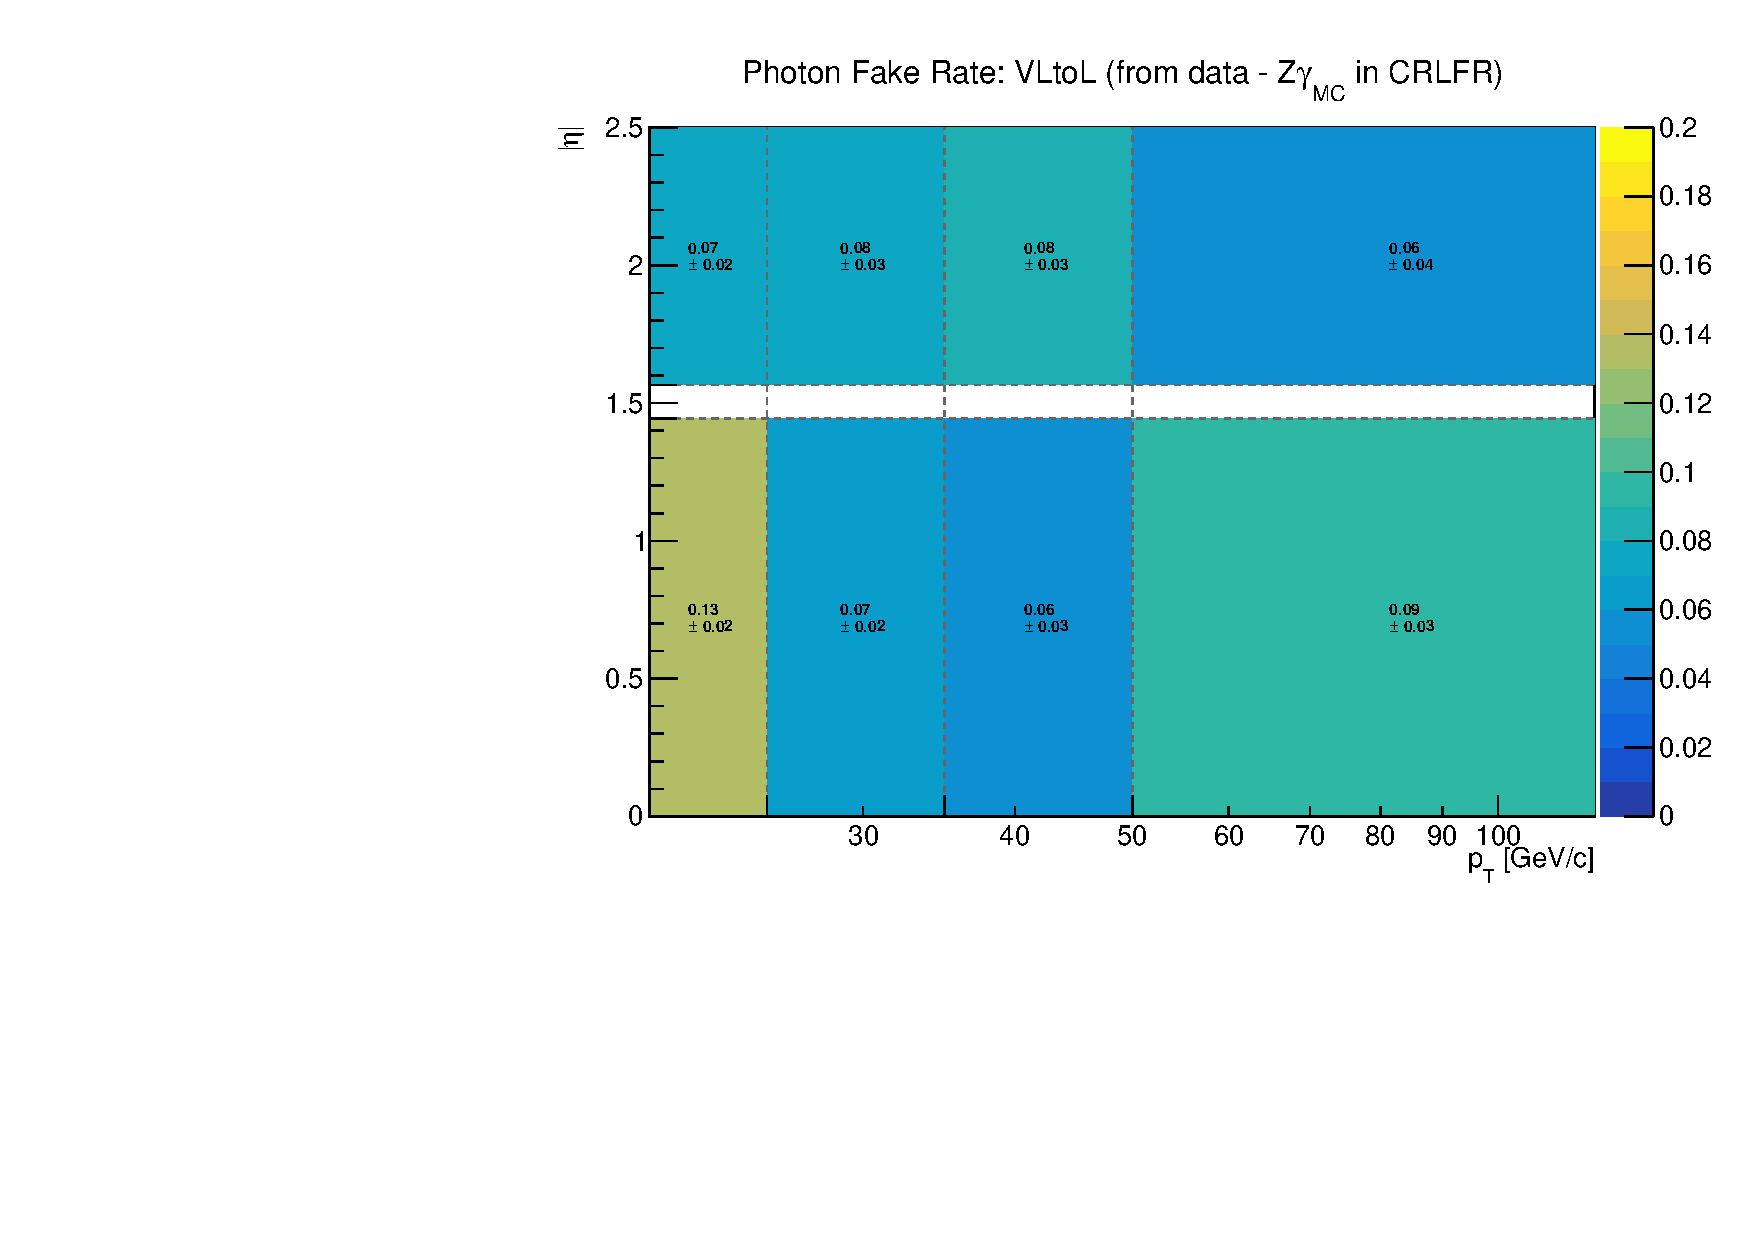
\includegraphics[width=.5\textwidth]{Figures/FR_VLtoL_pt-aeta_data-ZGToLLG_2016preVFP.pdf}}%
\subfigure [2016postVFP] {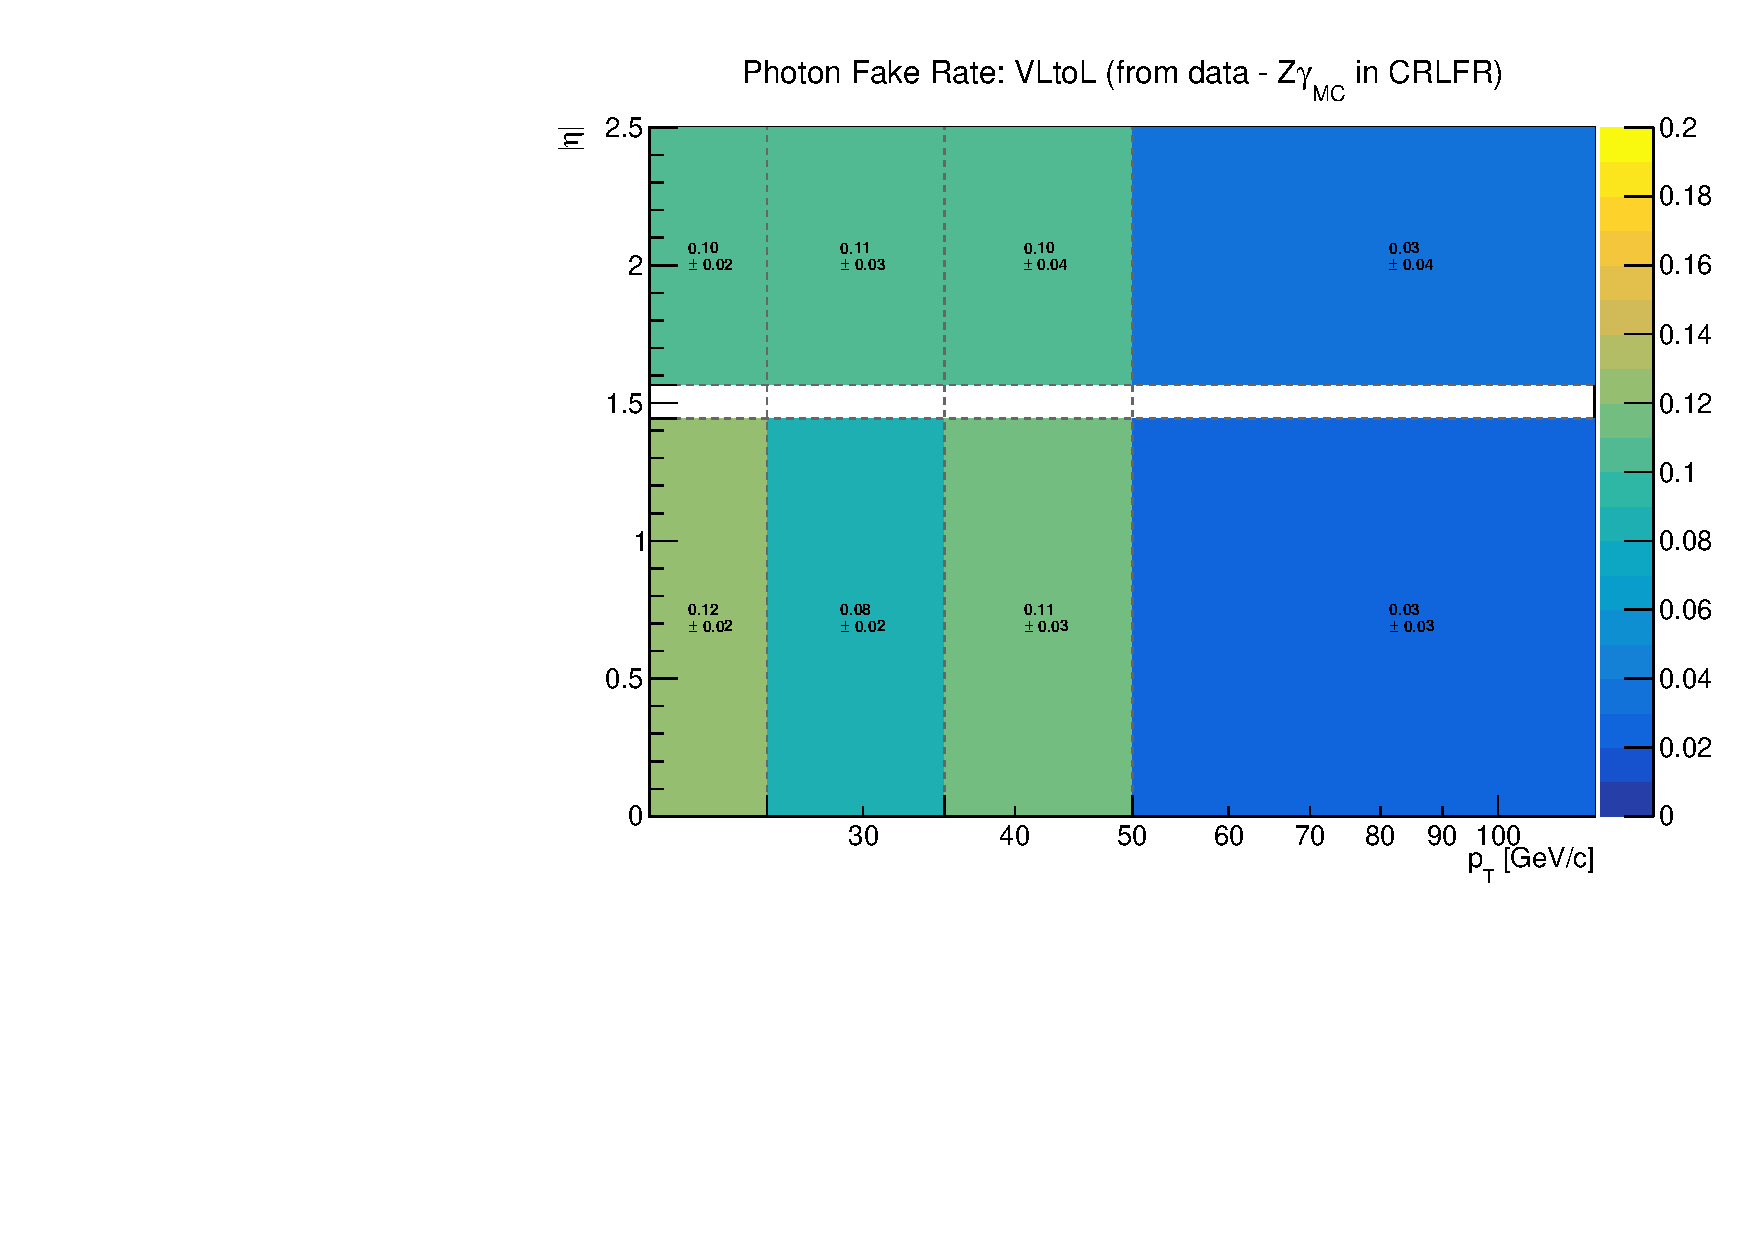
\includegraphics[width=.5\textwidth]{Figures/FR_VLtoL_pt-aeta_data-ZGToLLG_2016postVFP.pdf}}\\
\subfigure [2017]        {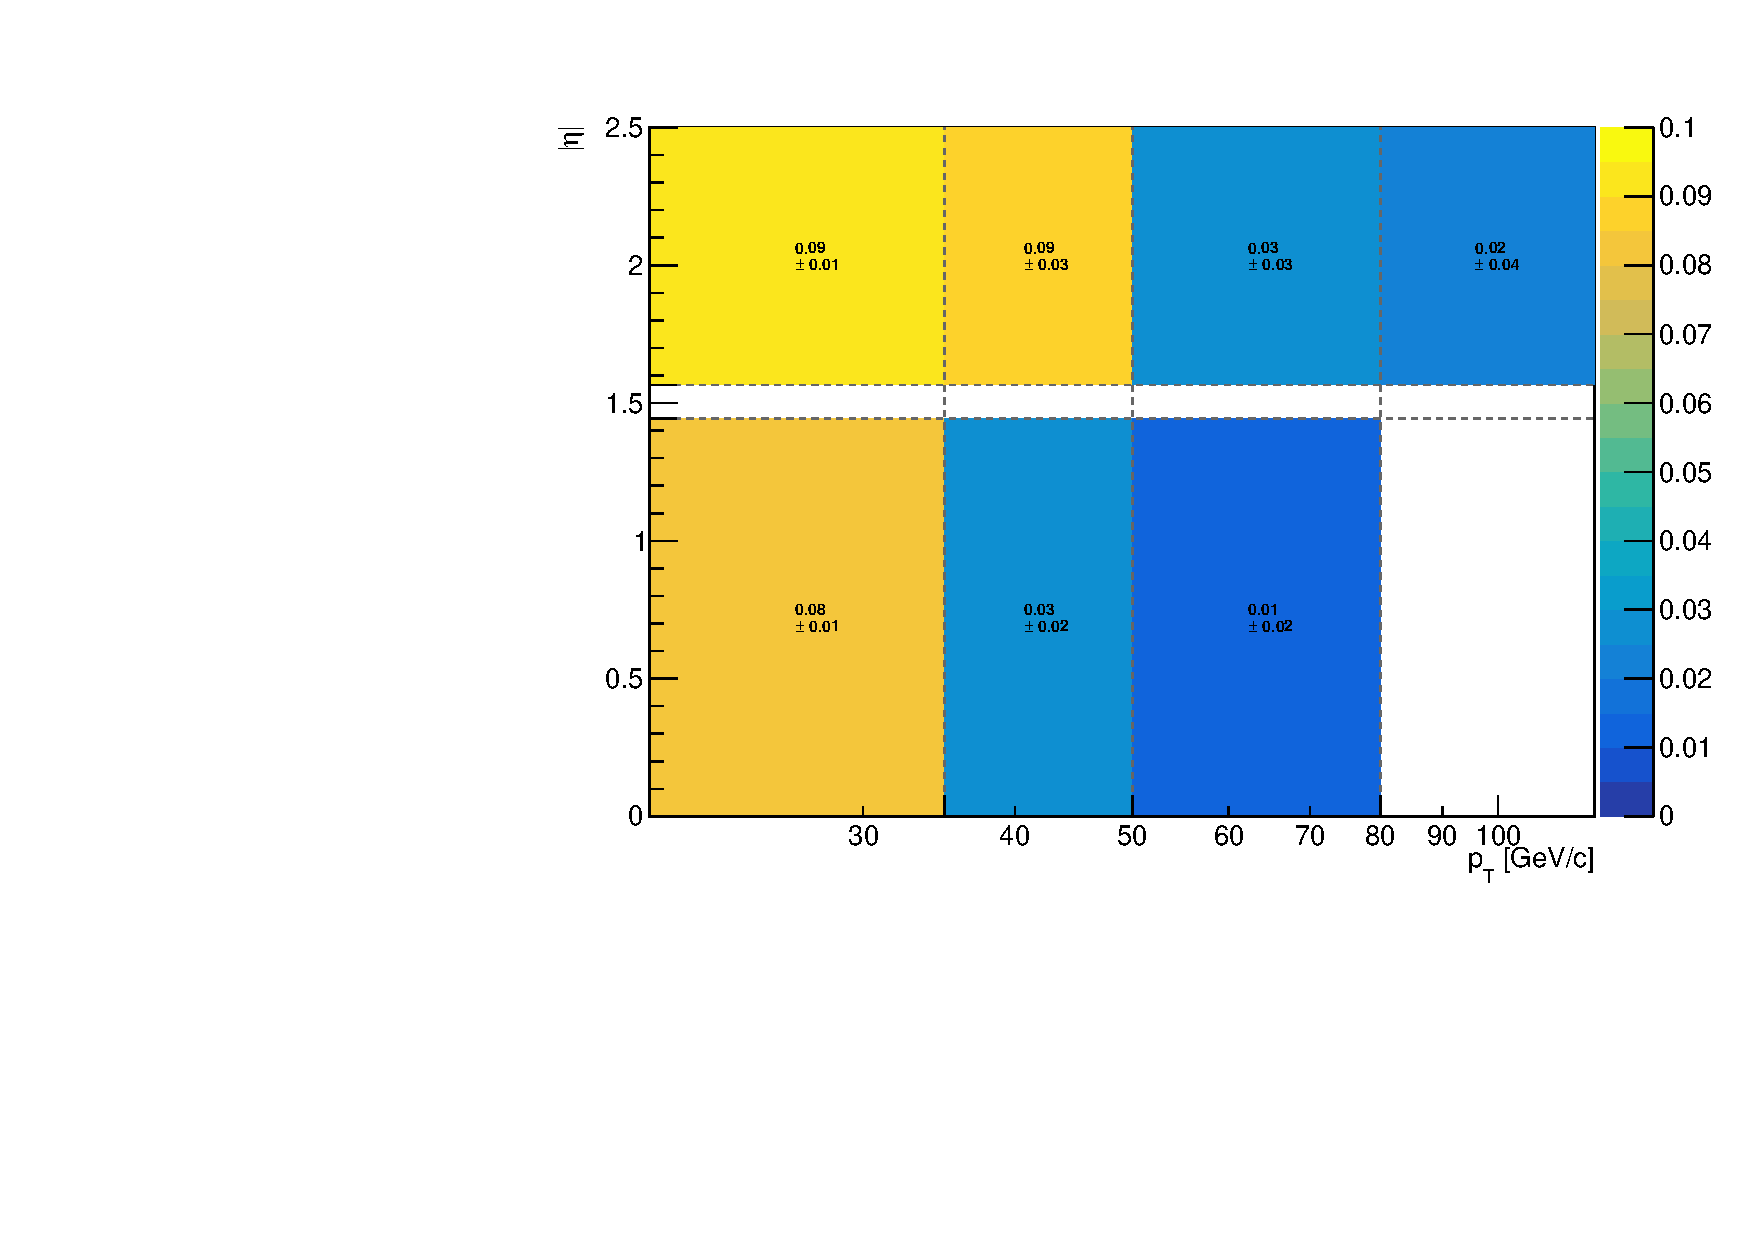
\includegraphics[width=.5\textwidth]{Figures/FR_VLtoL_pt-aeta_data-ZGToLLG_2017.pdf}}%
\subfigure [2018]        {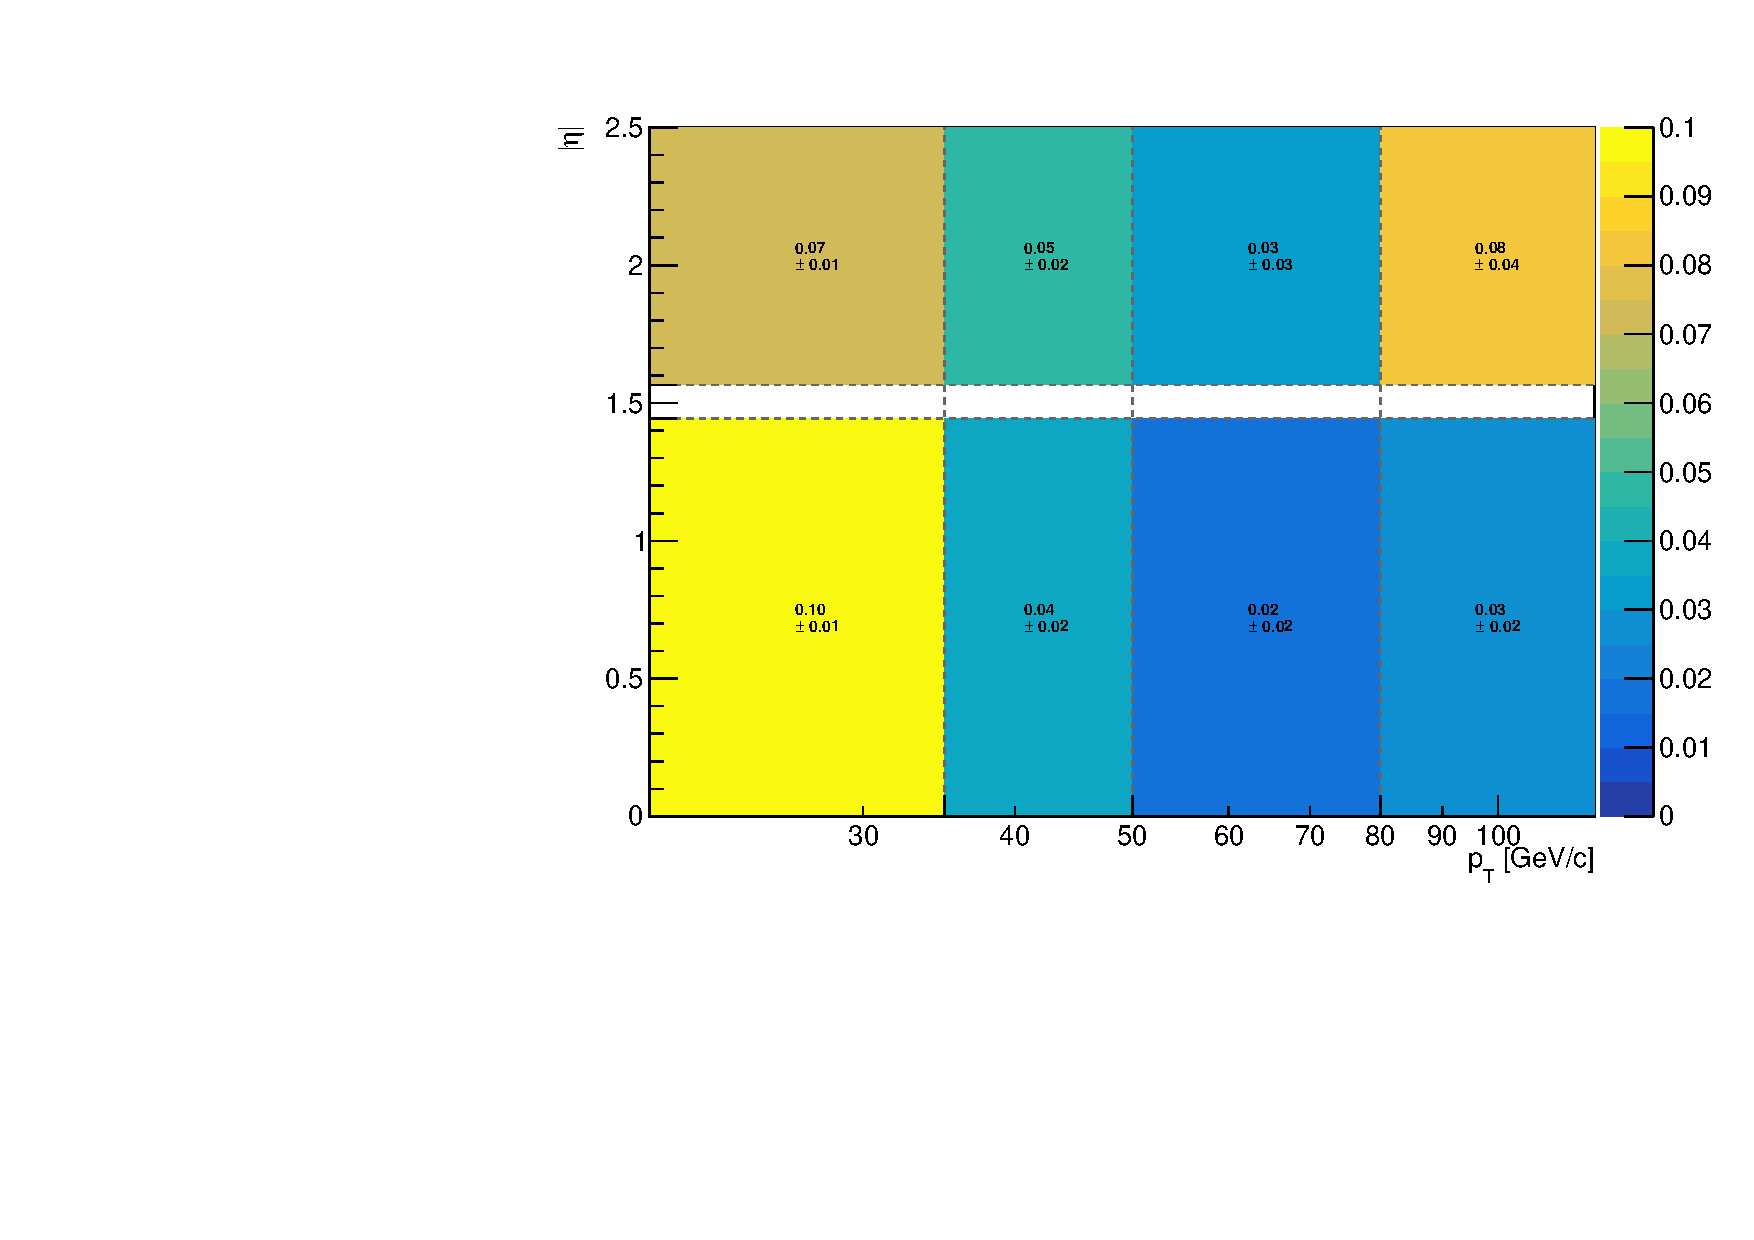
\includegraphics[width=.5\textwidth]{Figures/FR_VLtoL_pt-aeta_data-ZGToLLG_2018.pdf}}
\caption{Photon non-prompt rate as measured in data (with prompt $Z\gamma$ subtraction) using the cut-based ID for the photon.}
\label{fig:phFR_VLtoL}
\end{figure}

To ensure the stability of the measurement against other variables in the event,
additional measurements are carried out in specific sub-regions, and the results compared.
In particular, the effect of:
\begin{itemize}
\item The status of the third lepton: whether it passes or fails the tight selection.
  This could bias the measurement if the lepton were a misidentified jet and the additional hadronic activity produced an additional \nonprompt photon.
\item The flavour of the third lepton
\item The flavour of the SFOS pair that constitute the \PZ boson.
\item The number of additional jets in the event
\item The distance from the closest jet in the event
\end{itemize}

\note{Move to appendix? --> ``The results of these cross checks are in Appendix...''}

The photon non-prompt rate is assumed to be independent of the flavour of the leptons in the event.
This assumption is tested by deriving it separately for each flavour of the leptons of the Z boson $e^+ e^- \ell^\pm$ and $\mu^+ \mu^- \ell^\pm$, as shown in Figure \ref{fig:phFR_2e2m}.

\begin{figure}
\subfigure [$e^+ e^- \ell^\pm$]     {\resizebox{.5\textwidth}{!}{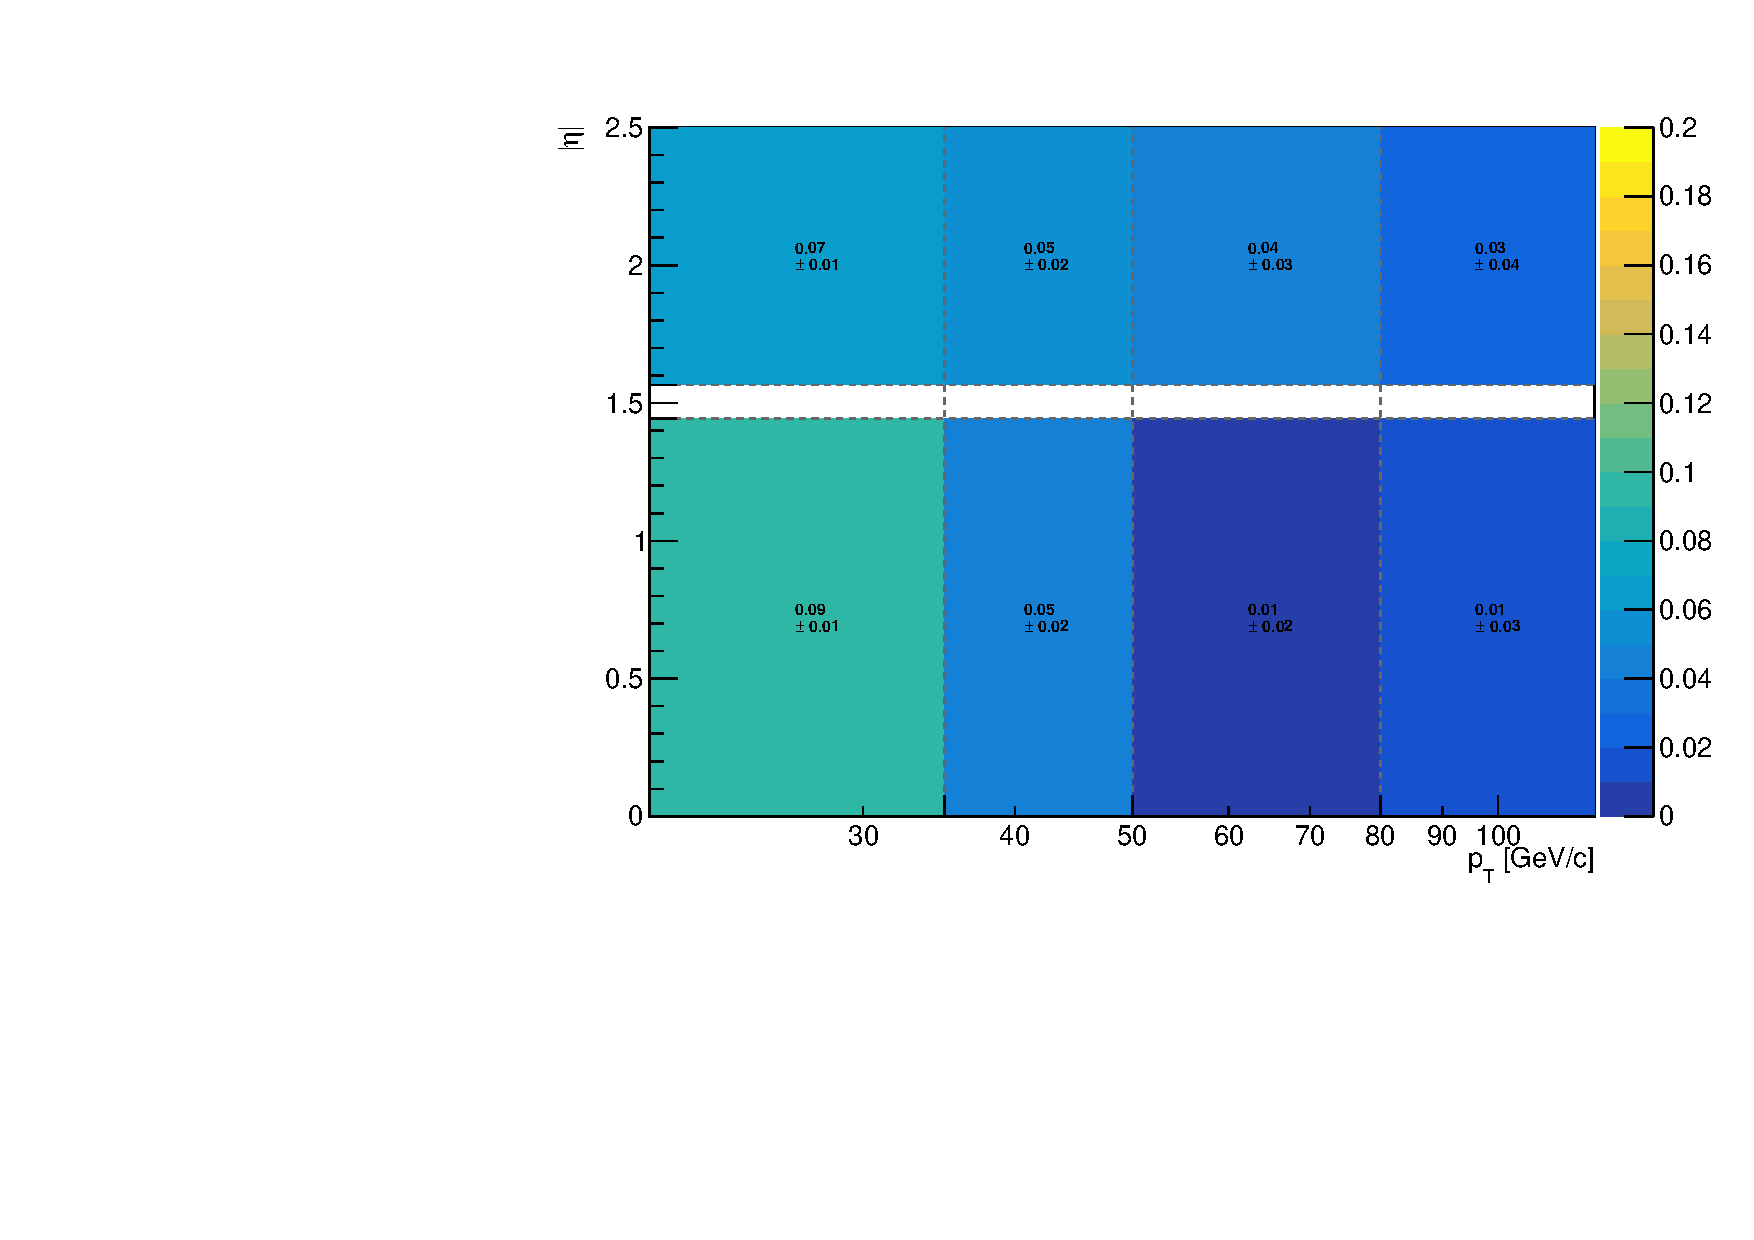
\includegraphics[width=.5\textwidth]{Figures/FR_VLtoL_pt-aeta_2e+x_data-ZGToLLG_2018.pdf}}}
\subfigure [$\mu^+ \mu^- \ell^\pm$] {\resizebox{.5\textwidth}{!}{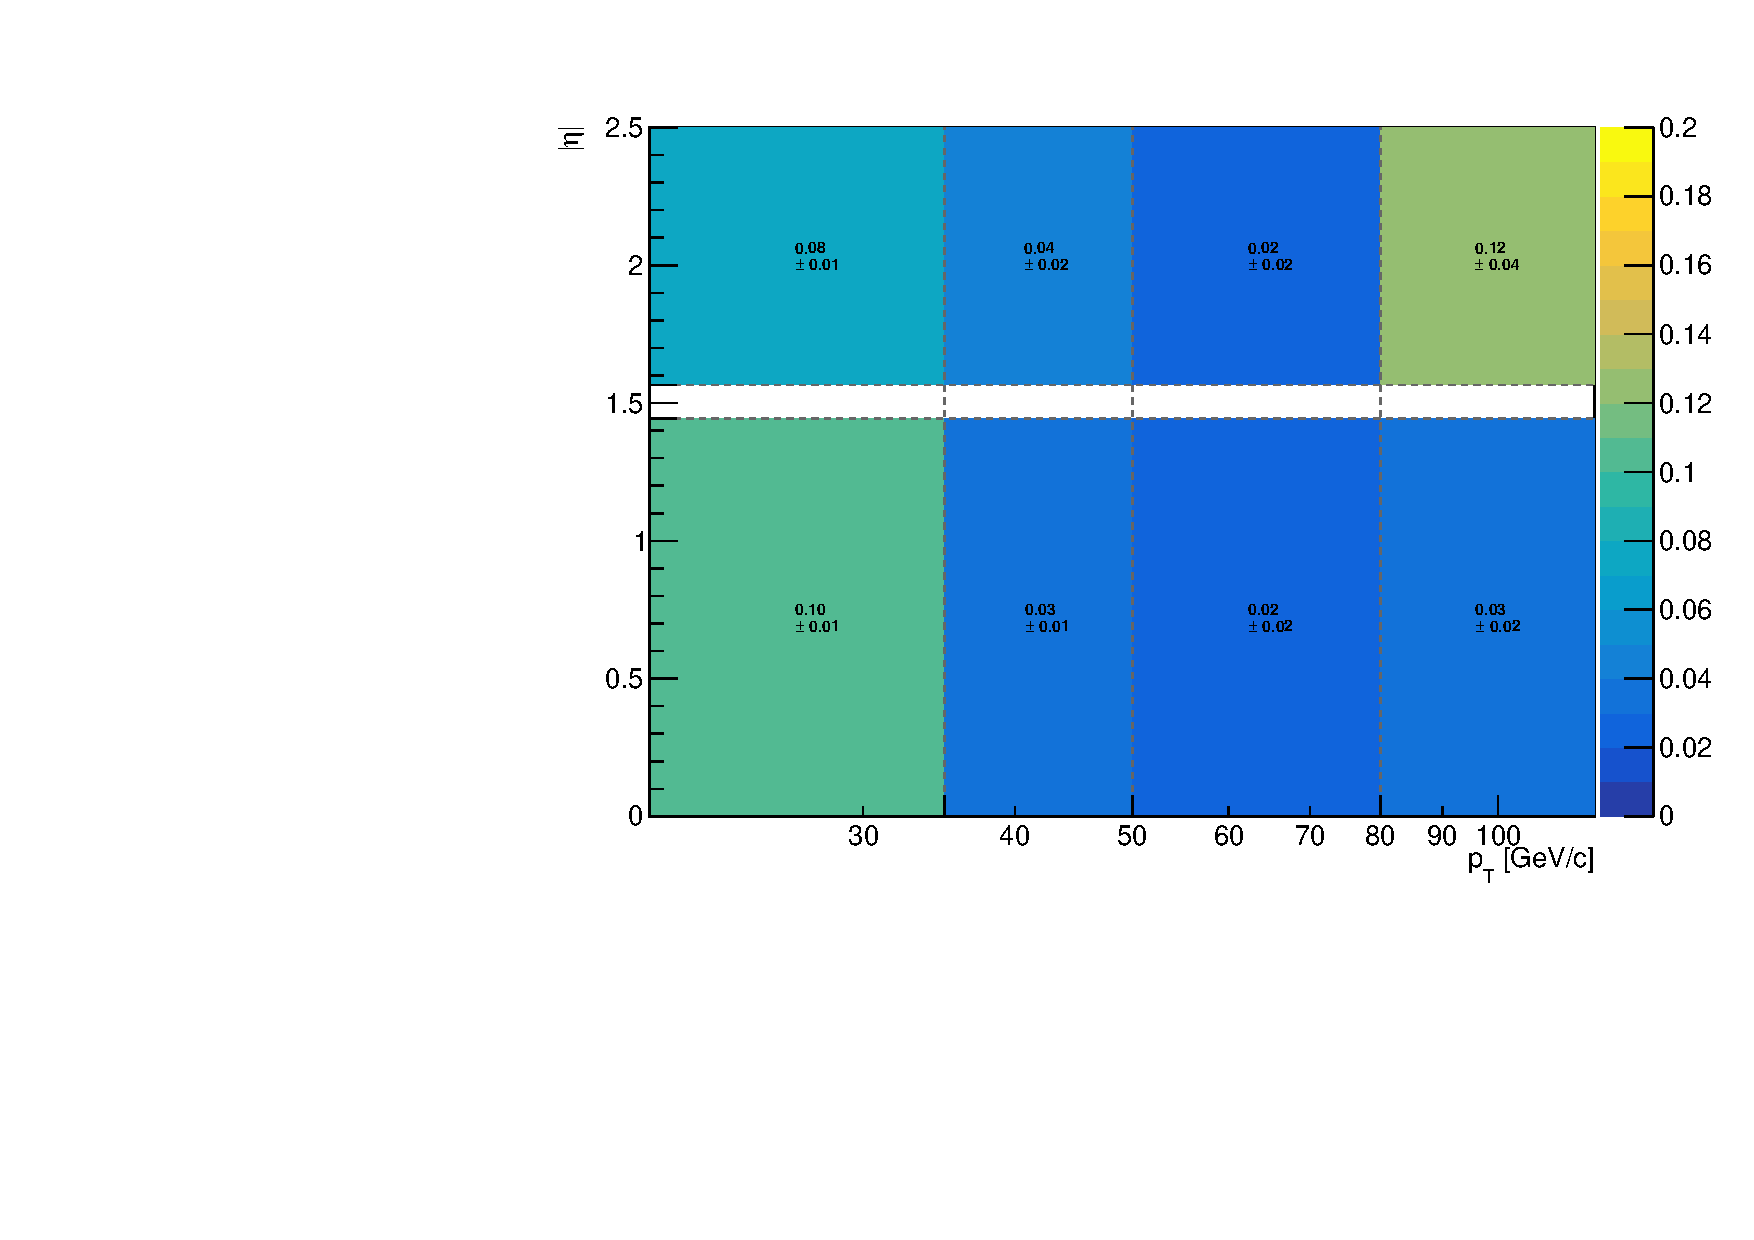
\includegraphics[width=.5\textwidth]{Figures/FR_VLtoL_pt-aeta_2m+x_data-ZGToLLG_2018.pdf}}}
\caption{Photon non-prompt rate as measured in 2018 data (with prompt $Z\gamma$ subtraction) in events with different lepton flavours for the Z boson.}
\label{fig:phFR_2e2m}
\end{figure}

The test is repeated for different flavours of the third lepton $\ell^+ \ell^- e^\pm$ and $\ell^+ \ell^- \mu^\pm$, and is shown in Figure \ref{fig:phFR_em}.

\begin{figure}
\subfigure [$\ell^+ \ell^- e^\pm$]   {\resizebox{.5\textwidth}{!}{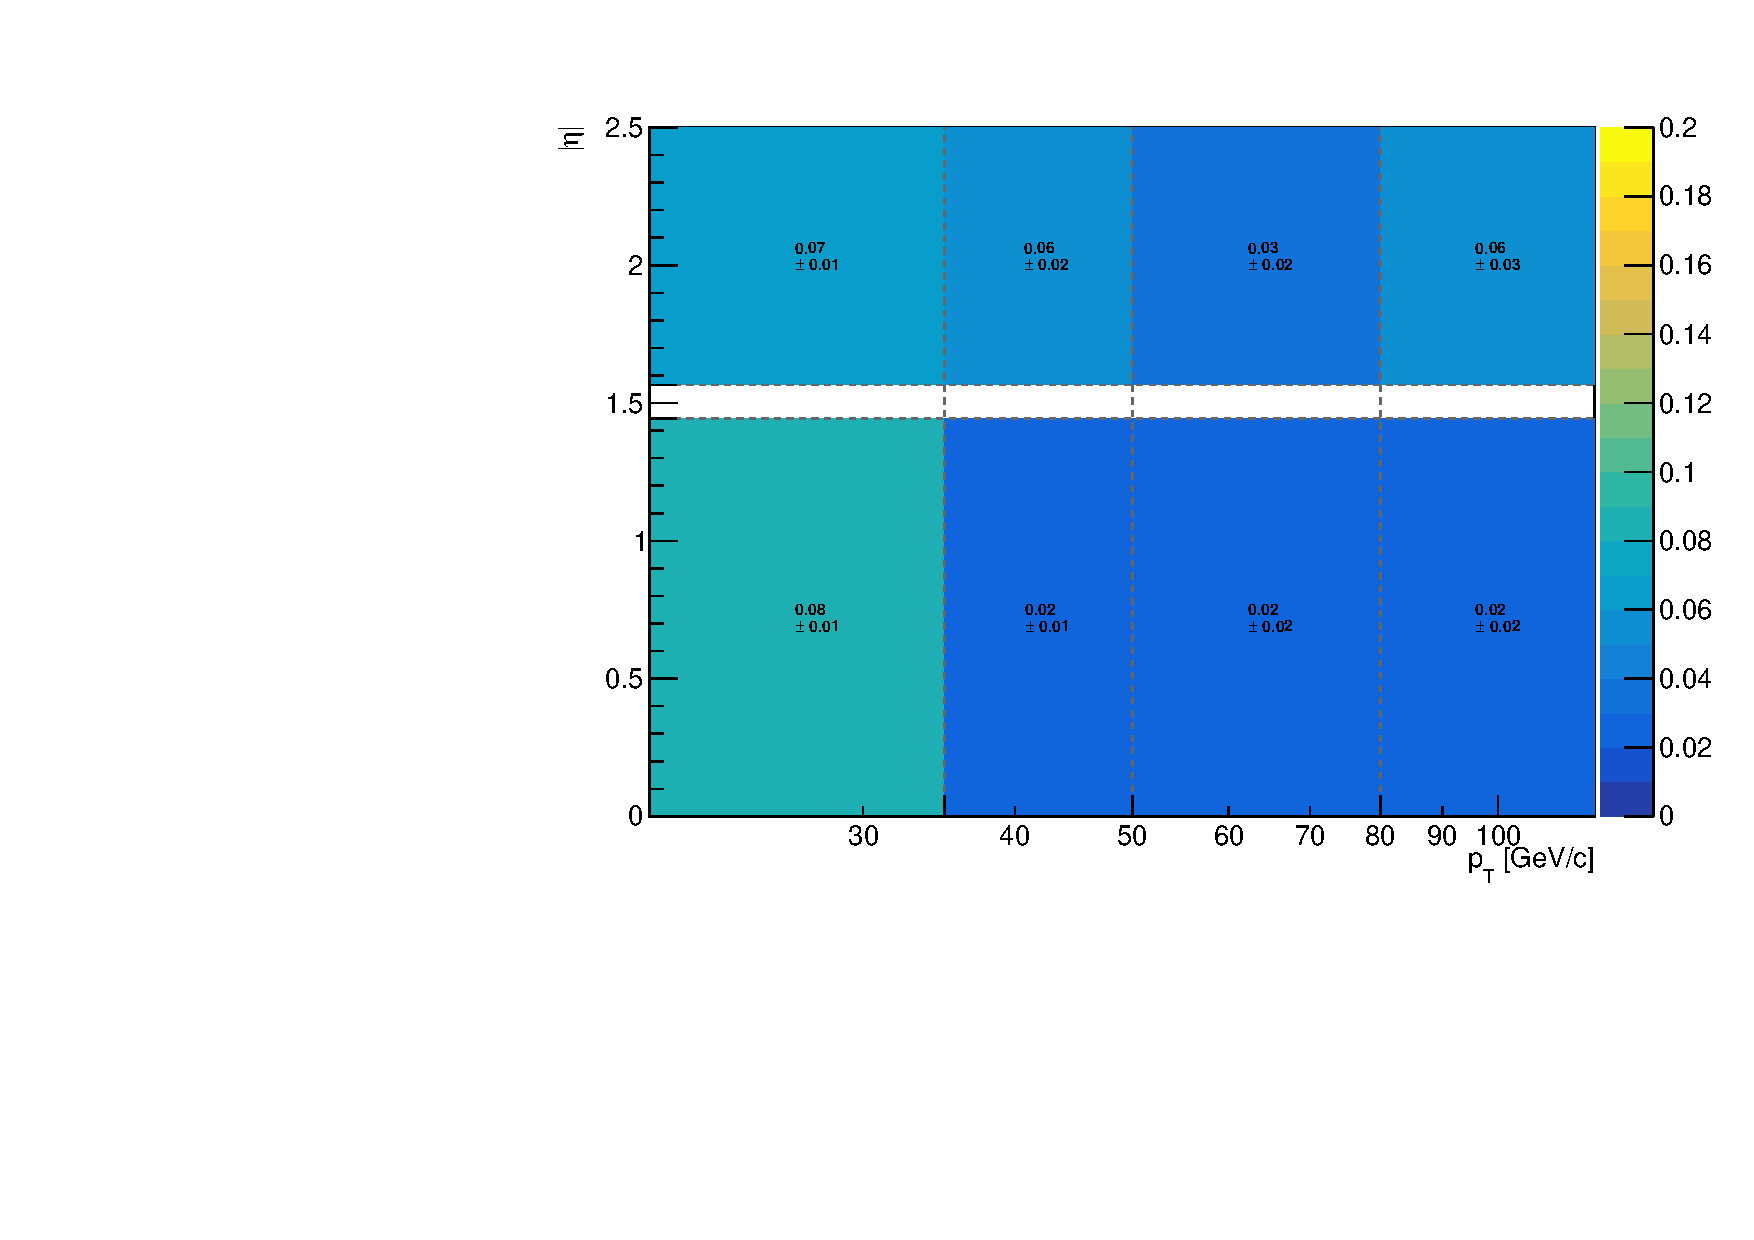
\includegraphics[width=.5\textwidth]{Figures/FR_VLtoL_pt-aeta_2x+e_data-ZGToLLG_2018.pdf}}}
\subfigure [$\ell^+ \ell^- \mu^\pm$] {\resizebox{.5\textwidth}{!}{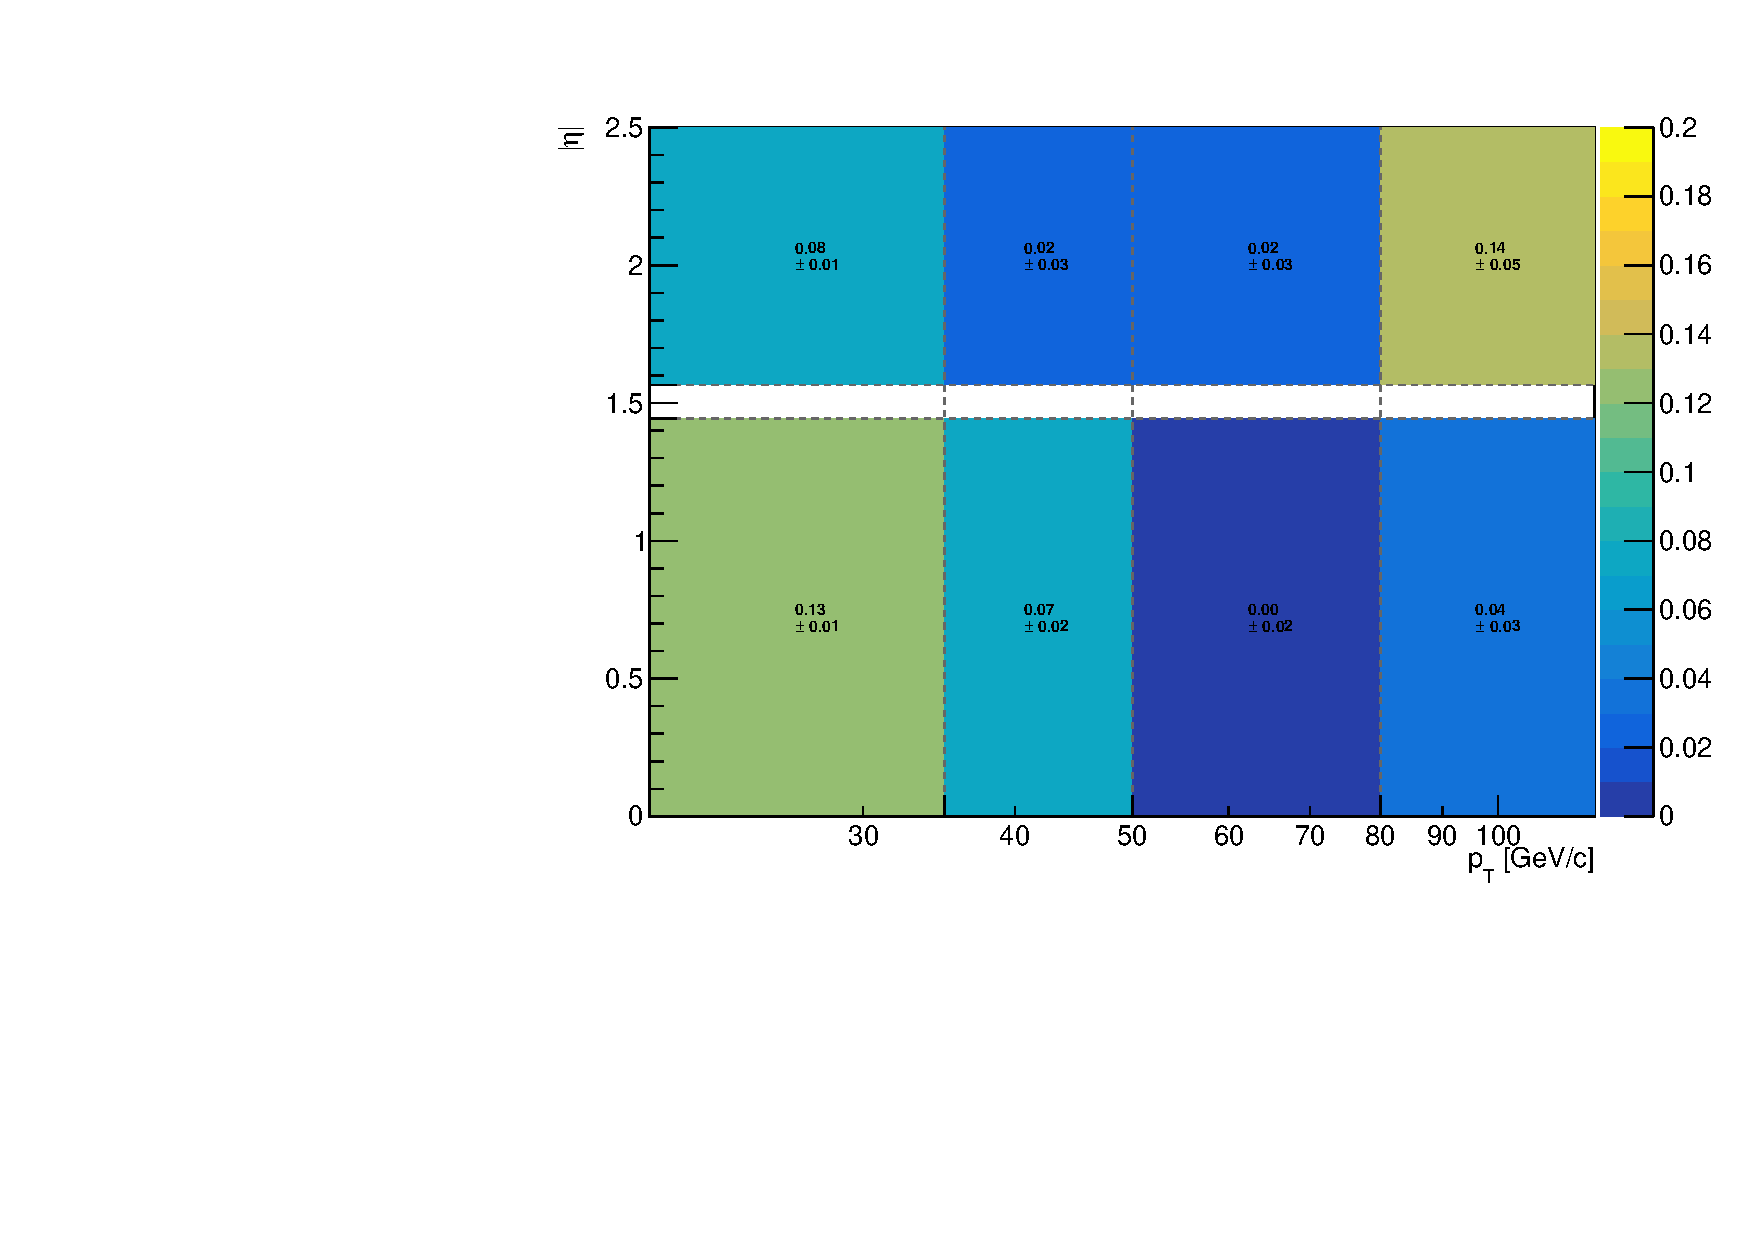
\includegraphics[width=.5\textwidth]{Figures/FR_VLtoL_pt-aeta_2x+m_data-ZGToLLG_2018.pdf}}}
\caption{Photon non-prompt rate as measured in 2018 data (with prompt $Z\gamma$ subtraction) in events with different flavours for the third lepton.}
\label{fig:phFR_em}
\end{figure}

Another test is performed by separating event where the third lepton passes/fails the tight analysis selection, shown in Figure \ref{fig:phFR_PF}.

\begin{figure}
\subfigure [$\ell^+ \ell^- \ell^\pm_{PASS}$] {\resizebox{.5\textwidth}{!}{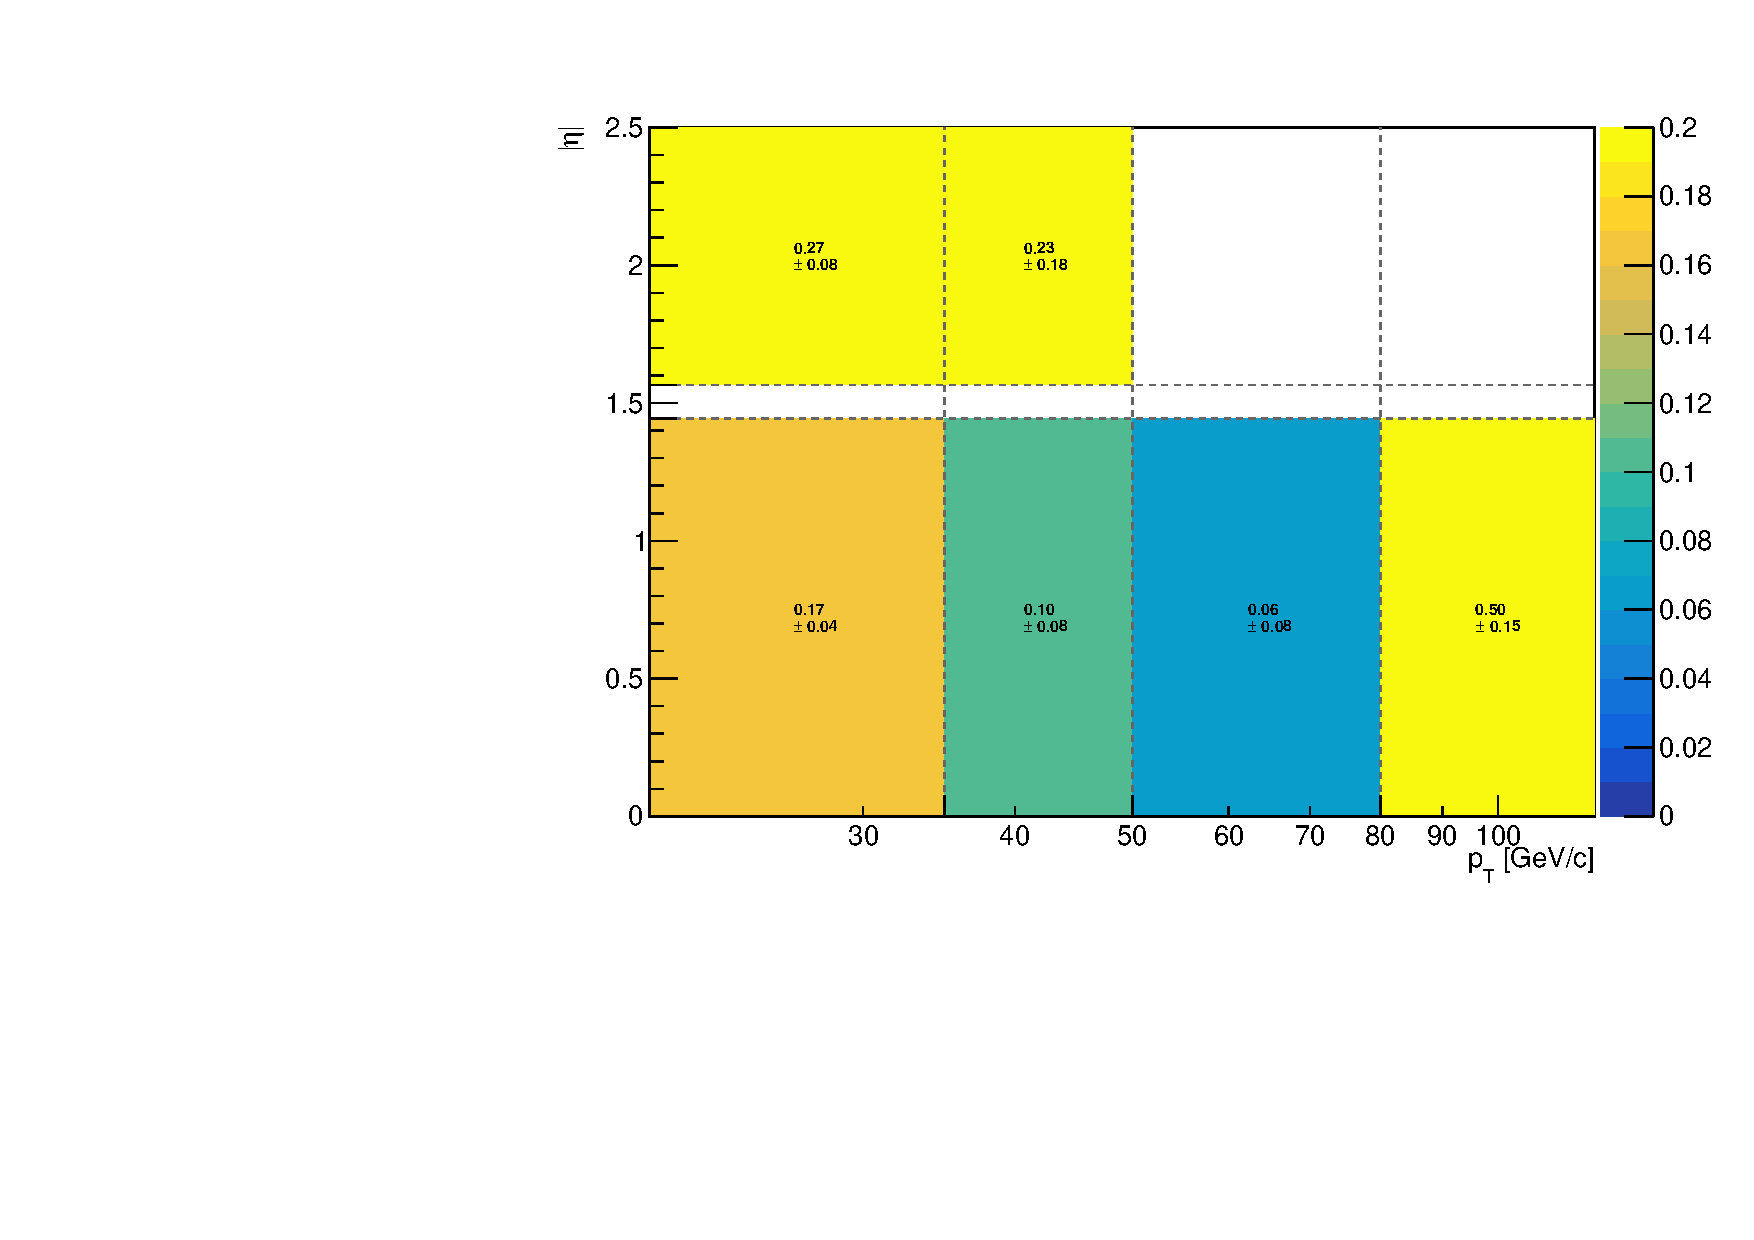
\includegraphics[width=.5\textwidth]{Figures/FR_VLtoL_pt-aeta_2x+P_data-ZGToLLG_2018.pdf}}}
\subfigure [$\ell^+ \ell^- \ell^\pm_{FAIL}$] {\resizebox{.5\textwidth}{!}{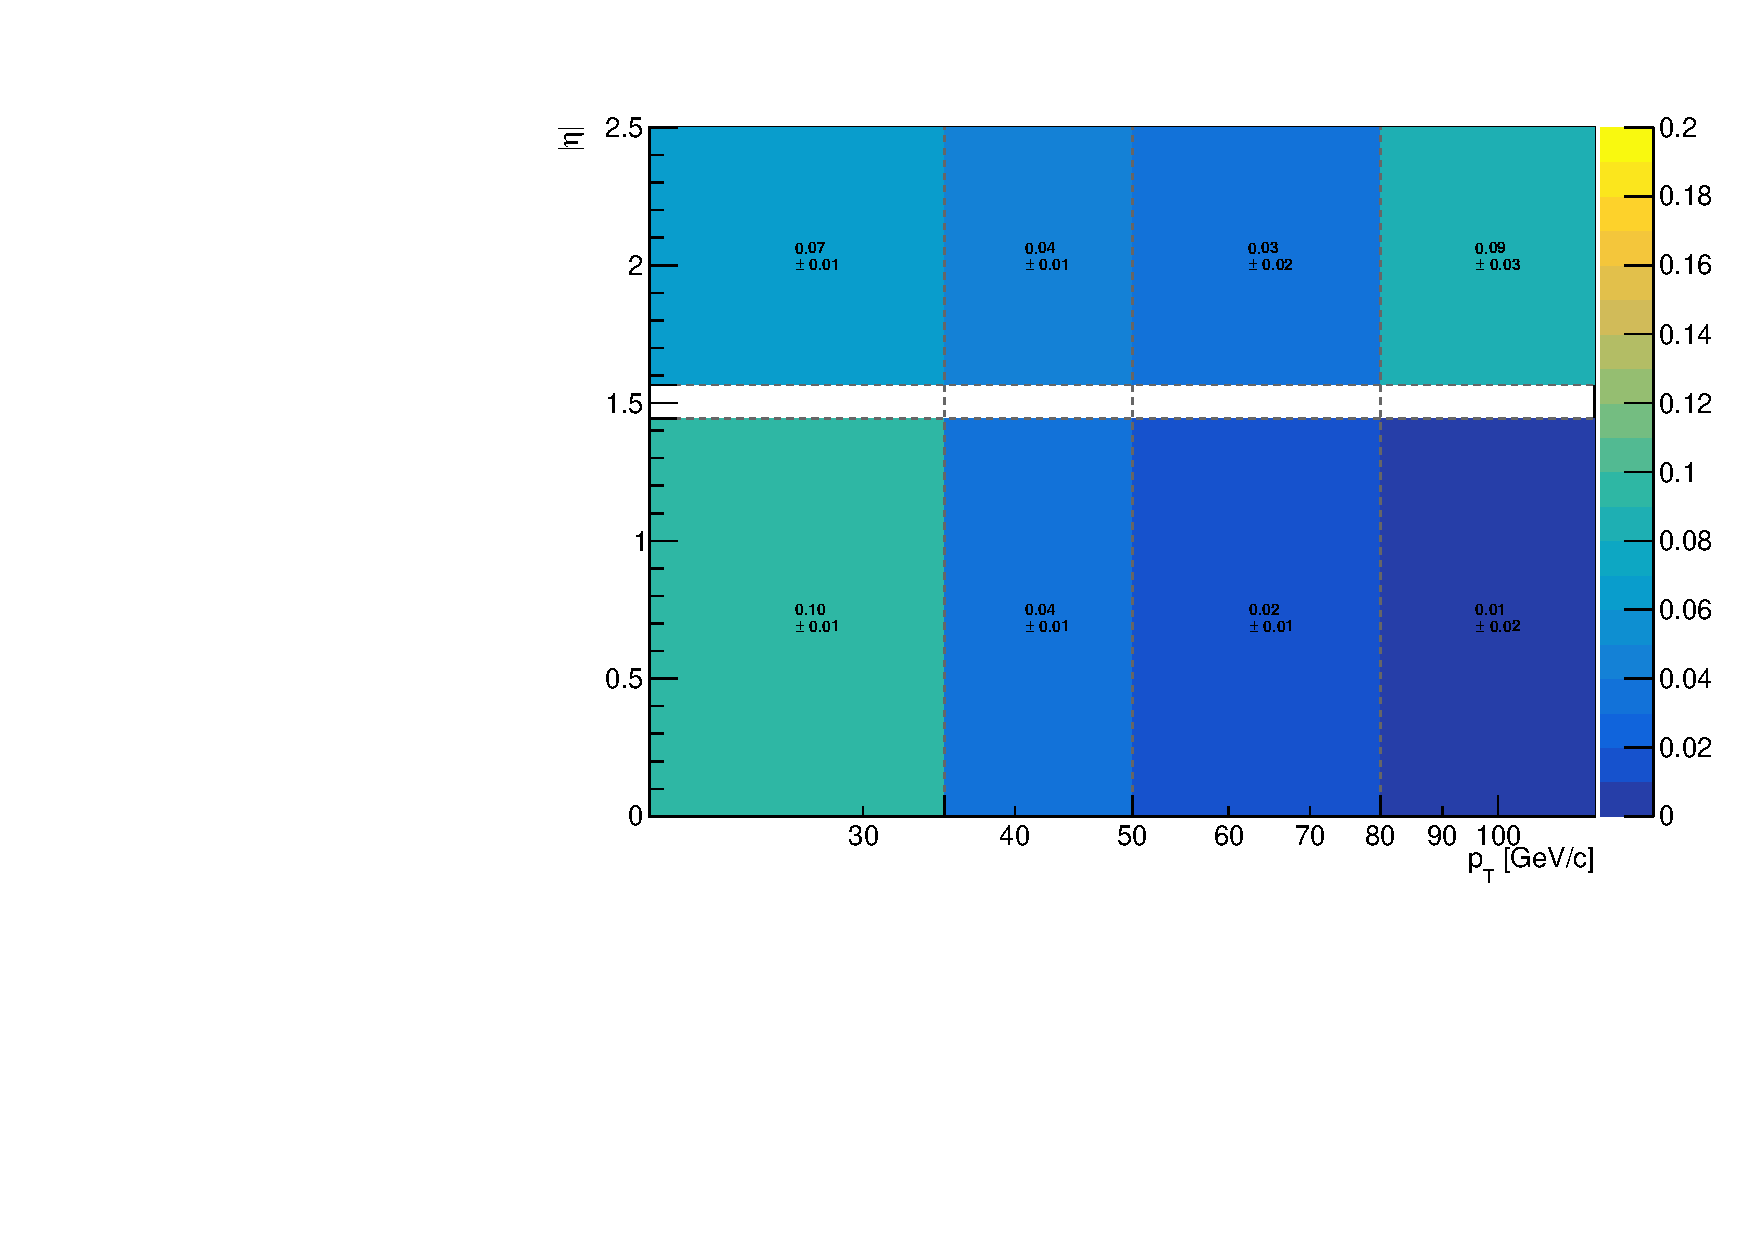
\includegraphics[width=.5\textwidth]{Figures/FR_VLtoL_pt-aeta_2x+F_data-ZGToLLG_2018.pdf}}}
\caption{Photon non-prompt rate as measured in 2018 data (with prompt $Z\gamma$ subtraction) in events where the third lepton passes/fails the tight selection, regardless of its flavour.}
\label{fig:phFR_PF}
\end{figure}

The trend for each $(p_{T}, |\eta|)$ bin for the different data-taking periods can be seen in Figure \ref{fig:phFR_time}.
It appears that, within the uncertainties, the measurements for each bin are compatible across the years and thus a single rate for the whole \Run2 could be derived.

\begin{figure}
\centering
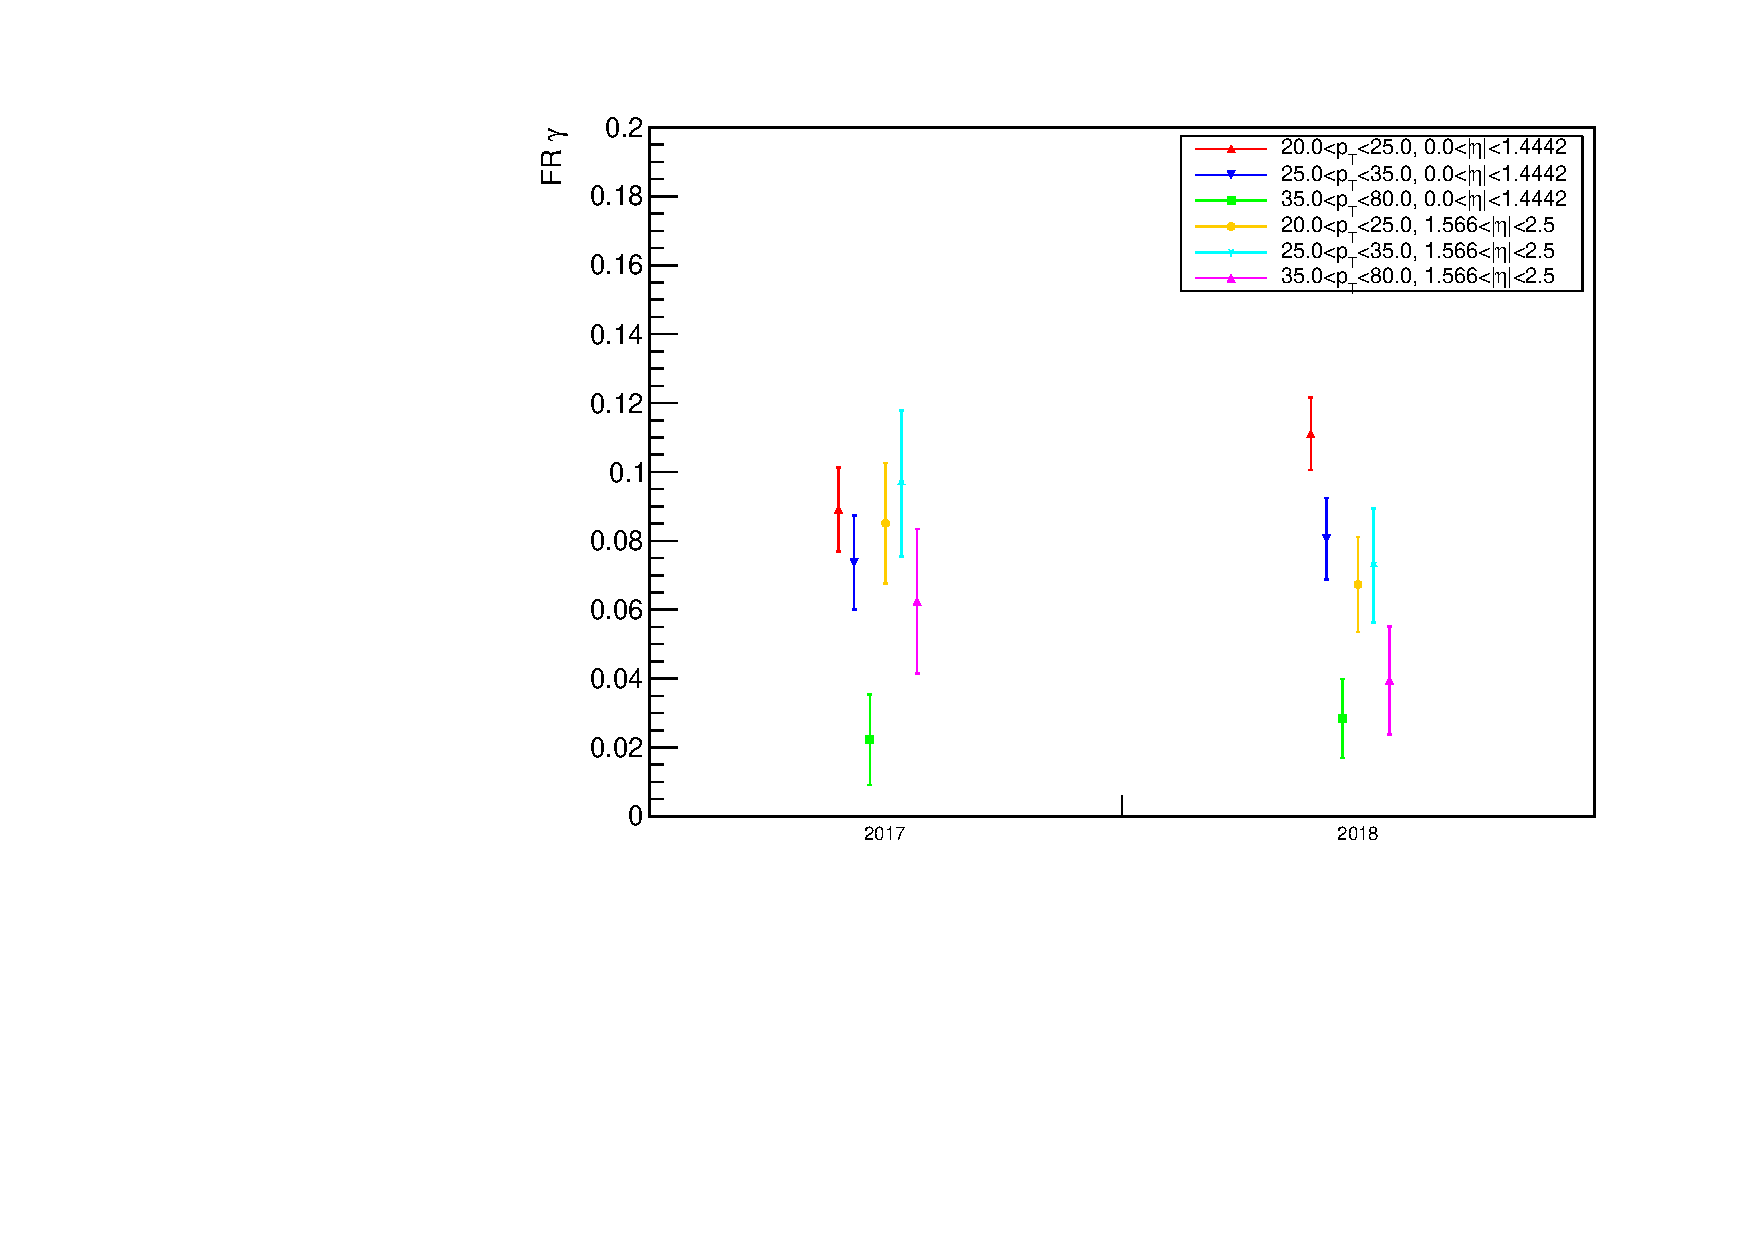
\includegraphics[width=.5\textwidth]{Figures/FR_VLtoL_pt-aeta_data-ZGToLLG_time.pdf}
\caption{Photon non-prompt rate in different data-taking periods.}
\label{fig:phFR_time}
\end{figure}

\subsubsection{Photon fake rate application}
The Fake Rate is then applied to events in the CR4P\_1F, CR3P\_1F and CR2P\_1F regions to estimate the non-prompt contribution in SR4P\_1P, SR3P\_1P, SR3P\_1P respectively.
Each event in this region is reweighed by the transfer factor $TF^\gamma(p_T, \eta) = \frac{f^\gamma}{1-f^\gamma}$, where $f^\gamma$ is the Fake Rate estimated in the measurement region.

\begin{equation}
  \begin{split}
    \label{eq:fakeRate_explanation_part1}
    N^{bkg}_{4P\_1P} &= \sum f_i N^{bkg}
    \\
    N^{bkg}_{4P\_1F} &= \sum ( 1-f_i ) N^{bkg}
  \end{split}
\end{equation}
where $N^{bkg}$ is the total number of events that have a fake photon, regardless of the region they are classified into.
From this it follows that the number of background events in the signal region is:
\begin{equation}
  \label{eq:fakeRate_explanation_part2}
  N^{bkg}_{4P\_1P} = \sum \frac{f_i}{1-f_i} N_{4P\_1F}
\end{equation}

\paragraph{Usage of the MVA based ID\\}
Additionally, kinematic photons that pass the MVA-based working points wp90 and wp80 are also considered,
given the improved performance of the MVA ID over the cut-based one.
The drawback is that this does not allow a data-driven estimation of the \nonprompt background,
due to the limited size of the application region defined by requiring a photon that passes the wp90 but fails the wp80.

Unlike a cut-based selection, it is not possible to invert only part of the MVA based ID.
The only way to derive a looser working point is to redo the optimisation of the raw MVA score,
and then study the efficiency of such selection in data and simulation to derive scale factors.
Both of these studies are outside the scope of this analysis.

Another possibility is to measure a fake rate between the kinematic selection and the looser MVA working point, \texttt{wp90}.
However, the former is too loose and the selected fakes have signatures that are very different from those of prompt photons.
This would make the assumption that the transfer factor is the same in the measurement and application regions quite unstable.

\todo{Add plots (e.g. Data/MC of CR3P1F/CR2P2F o SR4P blinded) of the number of events in wp90, wp80.}

Therefore, the results obtained using the MVA ID are derived without the data-driven estimate of fake photons.
In this case, the MC prediction of backgrounds which contain \nonprompt or misidentified photons is used.
